% ============================================================
%  Rapport PFA — Dental Reservation
%  Prêt pour Overleaf (pdfLaTeX)
%  Formatage : Times New Roman, 12pt corps, 1.5 interligne
% ============================================================
\documentclass[12pt, a4paper, oneside]{report}

% ---- Encodage & langue ----
\usepackage[utf8]{inputenc}
\usepackage[T1]{fontenc}
\usepackage[french]{babel}

% ---- Mise en page ----
\usepackage[top=3.5cm, bottom=2.5cm, left=2.5cm, right=2.5cm, headheight=1.8cm]{geometry}
\usepackage{setspace}
\onehalfspacing          % interligne 1.5 comme demandé

% ---- Police : Computer Modern (standard LaTeX) ----
\usepackage{lmodern}     % Latin Modern — version améliorée de Computer Modern

% ---- Couleurs & liens ----
\usepackage[dvipsnames,table]{xcolor}
\usepackage[hidelinks, colorlinks=true, linkcolor=black, urlcolor=blue, citecolor=black]{hyperref}

% ---- Graphiques ----
\usepackage{graphicx}
\graphicspath{{figures/}}
\usepackage{float}
\usepackage{subcaption}

% ---- Tableaux ----
\usepackage{array}
\usepackage{booktabs}
\usepackage{longtable}
\usepackage{tabularx}
\usepackage{multirow}

% ---- Listes ----
\usepackage{enumitem}

% ---- Code source ----
\usepackage{listings}
\usepackage{listingsutf8}
\lstset{
  basicstyle=\ttfamily\small,
  keywordstyle=\color{MidnightBlue}\bfseries,
  commentstyle=\color{OliveGreen}\itshape,
  stringstyle=\color{BrickRed},
  backgroundcolor=\color{gray!5},
  frame=single,
  rulecolor=\color{gray!40},
  breaklines=true,
  breakatwhitespace=true,
  tabsize=2,
  showstringspaces=false,
  captionpos=b,
  numbers=left,
  numberstyle=\tiny\color{gray},
  numbersep=8pt,
  xleftmargin=1.5em,
  framexleftmargin=1em,
  inputencoding=utf8,
  extendedchars=true,
  literate={é}{{\'e}}1 {è}{{\`e}}1 {ê}{{\^e}}1 {ë}{{\"e}}1
           {à}{{\`a}}1 {â}{{\^a}}1 {ù}{{\`u}}1 {û}{{\^u}}1
           {ô}{{\^o}}1 {î}{{\^i}}1 {ï}{{\"i}}1 {ç}{{\c{c}}}1
}

% ---- En-têtes & pieds de page ----
% Header: EMSI logo (left) | Chapter name (center) | Company logo (right)
% Page number at BOTTOM CENTER
\usepackage{fancyhdr}

% Define a teal/cyan color matching the EMSI template
\definecolor{emsiTeal}{RGB}{0, 128, 128}

\pagestyle{fancy}
\fancyhf{}                          % clear all
% ---- Header: logo left | chapter center | logo right ----
\fancyhead[L]{%
  
\includegraphics[height=1.2cm]{logo_emsi.png}%
}
\fancyhead[C]{%
  \footnotesize\textcolor{emsiTeal}{\leftmark}%
}
\fancyhead[R]{%
  
\includegraphics[height=1.2cm]{logo_company.png}%
}
% ---- Colored header rule ----
\renewcommand{\headrulewidth}{1.5pt}
\renewcommand{\headrule}{\hbox to\headwidth{%
  \color{emsiTeal}\leaders\hrule height \headrulewidth\hfill}}
% ---- Page number at bottom center ----
\fancyfoot[C]{\thepage}
\renewcommand{\footrulewidth}{0pt}

% ---- Ensure \leftmark persists on ALL pages of a chapter ----
% Override chaptermark so \leftmark = "Chapitre X : Title" (no uppercase)
\renewcommand{\chaptermark}[1]{%
  \markboth{\chaptername\ \thechapter\ : ##1}{}%
}
% Prevent \sectionmark from clearing \leftmark
\renewcommand{\sectionmark}[1]{}

% Plain style (chapter opening pages, TOC, etc.)
% Must mirror 'fancy' so the header with logos + chapter name appears on \chapter{} pages
\fancypagestyle{plain}{
  \fancyhf{}
  \fancyhead[L]{%
    
\includegraphics[height=1.2cm]{logo_emsi.png}%
  }
  \fancyhead[C]{%
    \footnotesize\textcolor{emsiTeal}{\leftmark}%
  }
  \fancyhead[R]{%
    
\includegraphics[height=1.2cm]{logo_company.png}%
  }
  \renewcommand{\headrulewidth}{1.5pt}
  \renewcommand{\headrule}{\hbox to\headwidth{%
    \color{emsiTeal}\leaders\hrule height \headrulewidth\hfill}}
  \fancyfoot[C]{\thepage}
  \renewcommand{\footrulewidth}{0pt}
}

% Chapter title page style: NO header, page number bottom center only
\fancypagestyle{chaptertitlepage}{
  \fancyhf{}
  \renewcommand{\headrulewidth}{0pt}
  \fancyfoot[C]{\thepage}
  \renewcommand{\footrulewidth}{0pt}
}

% ---- Table des matières cliquable ----
\usepackage[nottoc]{tocbibind}

% ---- Titre personnalisé pour les chapitres ----
% Titres des chapitres : gras 18pt, colored with line underneath
% Titres des paragraphes (sections) : gras 18pt
% Sous-paragraphes : normal
\usepackage{titlesec}

% Chapitre numéroté : colored title + decorative line (like in the EMSI template)
\titleformat{\chapter}[display]
  {\normalfont\fontsize{18}{22}\bfseries\color{emsiTeal}\centering}
  {\chaptertitlename\ \thechapter\ :}{0pt}
  {\fontsize{18}{22}\bfseries\color{emsiTeal}}
  [\vspace{4pt}{\color{emsiTeal}\titlerule[1.5pt]}]
\titlespacing*{\chapter}{0pt}{10pt}{30pt}

% Chapitre non numéroté (étoilé) : pour pages liminaires = 24pt gras centré
% NO header on liminary pages
\newcommand{\liminaryTitle}[1]{%
  \clearpage
  \thispagestyle{chaptertitlepage}
  \vspace*{2cm}
  \begin{center}
    {\fontsize{24}{29}\selectfont\bfseries #1}
  \end{center}
  \vspace{1.5cm}
}

% Section : gras 18pt
\titleformat{\section}
  {\normalfont\fontsize{18}{22}\bfseries}
  {\thesection}{1em}{}
\titlespacing*{\section}{0pt}{20pt}{10pt}

% Subsection : gras 14pt
\titleformat{\subsection}
  {\normalfont\fontsize{14}{17}\bfseries}
  {\thesubsection}{1em}{}
\titlespacing*{\subsection}{0pt}{15pt}{8pt}

% Subsubsection : normal 12pt
\titleformat{\subsubsection}
  {\normalfont\fontsize{12}{15}\selectfont}
  {\thesubsubsection}{1em}{}
\titlespacing*{\subsubsection}{0pt}{10pt}{5pt}

% ---- Légendes des figures : gras centré ----
\usepackage{caption}
\captionsetup[figure]{font=bf, justification=centering}
\captionsetup[table]{font=bf, justification=centering}

% ---- Métadonnées ----
\title{Application de Gestion de Cabinet Dentaire\\[0.3cm]\Large Dental Reservation}
\author{Projet de Fin d'Année (PFA)}
\date{Année universitaire 2025--2026}

% ============================================================
\begin{document}

% ---- Page de garde ----
% ============================================================
%  Page de Garde — Times New Roman
% ============================================================
\begin{titlepage}
\centering

\vspace*{1cm}

% ---- Logo de l'université (remplacer par votre logo) ----

\includegraphics[width=0.3\textwidth]{logo_emsi.png}\\[1cm]
{\fontsize{18}{22}\selectfont\bfseries EMSI --- École Marocaine des Sciences de l'Ingénieur}\\[0.3cm]
{\fontsize{14}{17}\selectfont Département d'Informatique}\\[2cm]

% ---- Titre ----
{\fontsize{24}{29}\selectfont\bfseries Rapport de Projet de Fin d'Année}\\[0.5cm]
{\fontsize{18}{22}\selectfont\bfseries (PFA)}\\[1.5cm]

{\fontsize{16}{20}\selectfont\itshape Application de Gestion de Cabinet Dentaire}\\[0.3cm]
{\fontsize{18}{22}\selectfont\bfseries Dental Reservation}\\[2cm]

% ---- Informations ----
\begin{minipage}{0.45\textwidth}
\begin{flushleft}
{\fontsize{14}{17}\selectfont\bfseries Réalisé par :}\\[0.3cm]
{\fontsize{14}{17}\selectfont
Prénom NOM\\
Prénom NOM}
\end{flushleft}
\end{minipage}
\hfill
\begin{minipage}{0.45\textwidth}
\begin{flushright}
{\fontsize{14}{17}\selectfont\bfseries Encadré par :}\\[0.3cm]
{\fontsize{14}{17}\selectfont
Pr. Prénom NOM}
\end{flushright}
\end{minipage}

\vfill

% ---- Année universitaire ----
{\fontsize{14}{17}\selectfont Année universitaire 2025 -- 2026}

\end{titlepage}


% ---- Pages liminaires (numérotation romaine) ----
\pagenumbering{roman}

% ============================================================
%  Dédicace — Gras centré 24pt Times New Roman
%  Texte centré 16pt italique Times New Roman
% ============================================================
\clearpage
\thispagestyle{empty}
\vspace*{\stretch{1}}

\begin{center}
{\fontsize{24}{29}\selectfont\bfseries Dédicace}
\end{center}

\vspace{2cm}

\begin{center}
{\fontsize{16}{20}\selectfont\itshape
À nos chers parents,\\[0.5cm]
qui ont toujours cru en nous et nous ont soutenus\\
tout au long de notre parcours académique.\\[0.5cm]
À nos familles et amis,\\[0.5cm]
pour leur amour, leur patience et leurs encouragements.\\[0.5cm]
À nos enseignants,\\[0.5cm]
pour les connaissances transmises et leur guidance précieuse.\\[0.5cm]
À tous ceux qui ont contribué, de près ou de loin,\\
à la réalisation de ce projet.
}
\end{center}

\vspace*{\stretch{2}}
\clearpage

% ============================================================
%  Remerciements — Gras centré 24pt Times New Roman
%  Texte centré 16pt italique Times New Roman
% ============================================================
\clearpage
\thispagestyle{empty}
\vspace*{\stretch{1}}

\begin{center}
{\fontsize{24}{29}\selectfont\bfseries Remerciements}
\end{center}

\vspace{2cm}

\begin{center}
{\fontsize{16}{20}\selectfont\itshape
Nous tenons à exprimer notre profonde gratitude\\
à toutes les personnes qui ont contribué,\\
directement ou indirectement, à la réalisation de ce projet.\\[0.8cm]
Nous remercions particulièrement notre encadrant\\
pour ses conseils avisés, son accompagnement méthodologique\\
et son soutien constant tout au long des différentes phases du projet.\\
Ses orientations ont été déterminantes dans la qualité finale du livrable.\\[0.8cm]
Nous remercions également l'ensemble du corps enseignant\\
pour les connaissances transmises durant notre formation,\\
qui ont constitué le socle technique sur lequel repose ce projet.\\[0.8cm]
Enfin, nous exprimons notre reconnaissance à nos proches\\
pour leur patience, leur compréhension\\
et leur encouragement tout au long de cette aventure.
}
\end{center}

\vspace*{\stretch{2}}
\clearpage

% ============================================================
%  Résumé — Titre gras centré 24pt Times New Roman
%  Corps 14pt Times New Roman
%  + Mots clés
% ============================================================
\clearpage
\thispagestyle{chaptertitlepage}

\vspace*{2cm}

\begin{center}
{\fontsize{24}{29}\selectfont\bfseries Résumé}
\end{center}

\vspace{1.5cm}

{\fontsize{14}{18}\selectfont
L'application \textbf{Dental Reservation} est une solution web complète destinée à optimiser la gestion quotidienne des cabinets dentaires. Elle couvre l'ensemble du cycle de vie d'un rendez-vous~: de l'authentification sécurisée du praticien jusqu'à la consultation du dossier médical du patient, en passant par la planification, la modification et la suppression des rendez-vous avec détection automatique des conflits de créneaux.

Le backend repose sur \textbf{ASP.NET Core 8} avec \textbf{Entity Framework Core} et une base de données \textbf{SQL Server}, exposant une API RESTful protégée par des jetons JWT. Le frontend est une application monopage \textbf{React 18 + TypeScript} construite avec \textbf{Vite}, stylisée avec \textbf{TailwindCSS} et la bibliothèque de composants \textbf{shadcn/ui}. Le déploiement est assuré par \textbf{Docker} et \textbf{Docker Compose} avec un proxy inverse \textbf{Nginx}.
}

\vspace{1.5cm}

{\fontsize{14}{18}\selectfont
\textbf{Mots clés :} Application web, Cabinet dentaire, Gestion de rendez-vous, ASP.NET Core, React, TypeScript, JWT, Entity Framework Core, SQL Server, Docker, API REST, TailwindCSS, shadcn/ui.
}

\clearpage

% ============================================================
%  Abstract — Titre gras centré 24pt Times New Roman
%  Corps 14pt Times New Roman
%  + Keywords
% ============================================================
\clearpage
\thispagestyle{chaptertitlepage}

\vspace*{2cm}

\begin{center}
{\fontsize{24}{29}\selectfont\bfseries Abstract}
\end{center}

\vspace{1.5cm}

{\fontsize{14}{18}\selectfont
The \textbf{Dental Reservation} application is a full-stack web solution designed to streamline the management of dental clinics. It provides secure JWT-based authentication, comprehensive patient record management (CRUD operations on the \texttt{pop\_personne} table), appointment scheduling with real-time conflict detection, calendar visualization with a weekly grid, available slots management, and an administration dashboard with key performance indicators.

The backend is built with \textbf{ASP.NET Core 8} and \textbf{Entity Framework Core} connected to a \textbf{SQL Server} database, exposing a RESTful API secured by JWT Bearer tokens. The frontend is a \textbf{React 18} single-page application written in \textbf{TypeScript}, bundled with \textbf{Vite}, styled with \textbf{TailwindCSS}, and powered by \textbf{shadcn/ui} component library. The two tiers communicate via HTTP, with the Vite dev server proxying \texttt{/api} requests to the backend. Docker and Docker Compose are used for containerized deployment with an Nginx reverse proxy.
}

\vspace{1.5cm}

{\fontsize{14}{18}\selectfont
\textbf{Keywords:} Web application, Dental clinic, Appointment management, ASP.NET Core, React, TypeScript, JWT, Entity Framework Core, SQL Server, Docker, REST API, TailwindCSS, shadcn/ui.
}

\clearpage

% ============================================================
%  Glossaire — Titre gras centré 24pt Times New Roman
%  Tri par ordre alphabétique
% ============================================================
\clearpage
\thispagestyle{chaptertitlepage}

\vspace*{2cm}

\begin{center}
{\fontsize{24}{29}\selectfont\bfseries Glossaire}
\end{center}
\addcontentsline{toc}{chapter}{Glossaire}

\vspace{1.5cm}

\begin{longtable}{@{} l p{12cm} @{}}
\toprule
\textbf{Acronyme} & \textbf{Signification} \\
\midrule
\endfirsthead
\toprule
\textbf{Acronyme} & \textbf{Signification} \\
\midrule
\endhead
\bottomrule
\endfoot
API     & Application Programming Interface \\
CI/CD   & Continuous Integration / Continuous Deployment \\
CORS    & Cross-Origin Resource Sharing \\
CRUD    & Create, Read, Update, Delete \\
CSS     & Cascading Style Sheets \\
DTO     & Data Transfer Object \\
EF Core & Entity Framework Core \\
EMSI    & École Marocaine des Sciences de l'Ingénieur \\
HMR     & Hot Module Replacement \\
HTML    & HyperText Markup Language \\
HTTPS   & HyperText Transfer Protocol Secure \\
JWT     & JSON Web Token \\
ORM     & Object-Relational Mapping \\
PFA     & Projet de Fin d'Année \\
REST    & Representational State Transfer \\
SPA     & Single Page Application \\
SQL     & Structured Query Language \\
UI      & User Interface \\
UML     & Unified Modeling Language \\
\end{longtable}

\clearpage


% ---- Liste des figures (no header) ----
\liminaryTitle{Liste des figures}
\addcontentsline{toc}{chapter}{Liste des figures}
\pagestyle{chaptertitlepage}
\listoffigures
\clearpage

% ---- Liste des tableaux (no header) ----
\liminaryTitle{Liste des tableaux}
\addcontentsline{toc}{chapter}{Liste des tableaux}
\pagestyle{chaptertitlepage}
\listoftables
\clearpage

% ---- Table des matières (no header) ----
\liminaryTitle{Table des matières}
\addcontentsline{toc}{chapter}{Table des matières}
\pagestyle{chaptertitlepage}
\tableofcontents
\clearpage

% Restore normal header for the rest of the document
\pagestyle{fancy}

% ---- Corps du rapport (numérotation arabe) ----
\pagenumbering{arabic}

% ============================================================
%  Introduction Générale
%  Corps : 12pt Times New Roman, interligne 1.5
% ============================================================
\clearpage


\vspace*{2cm}

\begin{center}
{\fontsize{24}{29}\selectfont\bfseries Introduction Générale}
\end{center}
\addcontentsline{toc}{chapter}{Introduction Générale}

\vspace{1.5cm}

La gestion d'un cabinet dentaire implique un ensemble de processus complexes~: la prise de rendez-vous, la gestion des dossiers patients, le suivi des praticiens et l'administration des créneaux horaires. Les systèmes traditionnels, souvent basés sur des registres papier ou des tableurs, présentent des limitations significatives en termes de fiabilité, de traçabilité et d'efficacité.

Dans un cabinet dentaire, la planification des rendez-vous est une tâche critique. Une mauvaise gestion peut entraîner des conflits de créneaux (deux patients programmés chez le même médecin à la même heure), des temps d'attente excessifs, des oublis de rendez-vous, et une sous-utilisation des ressources (cabinets vides). Ces problématiques affectent directement la qualité du service et la satisfaction des patients.

Par ailleurs, les dossiers patients --- contenant les informations personnelles, les antécédents médicaux, les contrats d'assurance et l'historique des consultations --- doivent être centralisés, sécurisés et facilement accessibles pour permettre un suivi efficace.

Dans ce contexte, le présent projet vise à concevoir et réaliser une application web moderne baptisée \textbf{Dental Reservation}, capable de répondre à l'ensemble de ces besoins. L'application offre une interface intuitive permettant aux praticiens de gérer leurs patients, planifier et modifier les rendez-vous avec détection automatique des conflits, visualiser les créneaux disponibles sur un calendrier hebdomadaire, et consulter les dossiers médicaux --- le tout de manière sécurisée grâce à un mécanisme d'authentification par jeton JWT.

Ce rapport décrit le projet dans son intégralité~:

\begin{itemize}
    \item \textbf{Chapitre 1} présente le contexte général, l'organisme d'accueil et un aperçu de la solution.
    \item \textbf{Chapitre 2} détaille l'étude fonctionnelle et technique~: architecture, besoins et spécifications.
    \item \textbf{Chapitre 3} couvre la conception UML avec les diagrammes de cas d'utilisation, de classes, de séquence et d'activité.
    \item \textbf{Chapitre 4} présente la réalisation, avec une description détaillée de chaque module et fonctionnalité de l'application.
\end{itemize}

\clearpage

% ============================================================
%  Chapitre 1 : Contexte Général
%  Titres chapitres : gras 18pt
%  Titres paragraphes (sections) : gras 18pt
%  Sous-paragraphes : normal
%  Corps : 12pt Times New Roman, interligne 1.5
% ============================================================

% ---- Page de titre du chapitre ----
\clearpage
\thispagestyle{chaptertitlepage}
\vspace*{\fill}
\begin{center}
\rule{\textwidth}{0.4pt}\\[0.8cm]
{\fontsize{24}{29}\selectfont\bfseries Chapitre 1}\\[0.6cm]
{\fontsize{18}{22}\selectfont Contexte Général}\\[0.8cm]
\rule{\textwidth}{0.4pt}
\end{center}
\vspace*{\fill}
\clearpage

% ---- Contenu du chapitre ----
\chapter{Contexte Général}

\section{Introduction}

Ce chapitre présente le contexte général dans lequel s'inscrit le projet \textbf{Dental Reservation}. Il décrit l'organisme d'accueil, la problématique identifiée, les objectifs du projet et un aperçu de la solution développée.

\section{Organisme d'accueil}

Le projet a été réalisé dans le cadre d'un Projet de Fin d'Année (PFA) au sein d'un cabinet dentaire. L'organisme d'accueil est spécialisé dans la prestation de soins dentaires et la gestion des rendez-vous patients. L'objectif principal du stage était de moderniser le système de gestion existant en le remplaçant par une solution numérique performante et ergonomique.

Le cabinet gère quotidiennement un volume important de patients, de rendez-vous et de praticiens. Avant la mise en place de cette application, la gestion se faisait principalement à travers~:

\begin{itemize}
    \item Un registre papier pour les rendez-vous
    \item Des fiches cartonnées pour les dossiers patients
    \item Des appels téléphoniques pour la confirmation des rendez-vous
\end{itemize}

La nécessité d'un outil centralisé s'est imposée pour~:

\begin{itemize}
    \item \textbf{Éliminer les erreurs de planification}~: doublons de créneaux, conflits horaires entre médecins et cabinets
    \item \textbf{Centraliser les dossiers patients}~: accès instantané aux informations personnelles, aux contrats d'assurance et à l'historique des consultations
    \item \textbf{Offrir une vue calendaire claire} de la charge de travail de chaque praticien
    \item \textbf{Permettre un accès sécurisé} à l'application, réservé aux personnels autorisés
    \item \textbf{Automatiser les calculs}~: créneaux disponibles, statistiques, âge des patients
\end{itemize}

% ============================================================
\section{Présentation du projet}

L'application \textbf{Dental Reservation} est une plateforme web full-stack qui permet aux cabinets dentaires de gérer efficacement leurs opérations quotidiennes. Le système couvre les fonctionnalités suivantes~:

\subsection{Authentification et sécurité}
\begin{itemize}
    \item Connexion sécurisée par identifiant (email) et mot de passe
    \item Génération de jetons JWT avec une durée de validité d'une heure
    \item Protection de toutes les routes API par le middleware d'autorisation
    \item Stockage du token côté client dans le \texttt{localStorage} du navigateur
    \item Routes React protégées par un composant \texttt{ProtectedRoute} qui redirige les utilisateurs non authentifiés
\end{itemize}

\subsection{Gestion des patients}
\begin{itemize}
    \item Création de fiches patients avec informations complètes~: nom, prénom, date de naissance, sexe, CIN, matricule, code collectivité, adresse, email, téléphone
    \item Modification et suppression de patients existants
    \item Recherche dynamique par nom, prénom, téléphone, email ou matricule
    \item Consultation du dossier complet d'un patient avec son historique de rendez-vous, triés par date décroissante
    \item Export du dossier patient en PDF via la fonction d'impression du navigateur
    \item Statistiques sur le nombre total de patients actifs
\end{itemize}

\subsection{Gestion des rendez-vous}
\begin{itemize}
    \item Création de rendez-vous avec sélection du patient (via un composant Combobox recherchable), du médecin, du cabinet, de la date, de l'heure, de la durée et de la nature du soin
    \item Détection automatique des conflits de créneaux~: le serveur vérifie qu'aucun rendez-vous actif n'existe pour le même médecin ou le même cabinet à la même date et heure
    \item Modification du statut (confirmé, en attente, annulé) et des informations d'un rendez-vous
    \item Suppression de rendez-vous
    \item Filtrage par patient, médecin, date et statut
\end{itemize}

\subsection{Calendrier hebdomadaire}
\begin{itemize}
    \item Vue sur 7 jours (lundi à dimanche) avec navigation semaine par semaine
    \item Grille horaire de 08:00 à 17:30 avec pas de 30 minutes
    \item Affichage des rendez-vous dans les cellules avec code couleur selon le statut (vert = confirmé, jaune = en attente, rouge = annulé)
    \item Indicateur visuel de l'heure courante (ligne rouge) sur la colonne du jour
    \item Panneau latéral \og Today's Schedule \fg{} avec la liste des rendez-vous du jour
\end{itemize}

\subsection{Créneaux disponibles}
\begin{itemize}
    \item Grille visuelle des créneaux horaires avec distinction disponible/réservé
    \item Durée configurable du créneau (15, 30, 45 ou 60 minutes)
    \item Statistiques de remplissage~: total de créneaux, disponibles, réservés, taux d'utilisation
    \item Réservation rapide au clic sur un créneau disponible
\end{itemize}

\subsection{Profil utilisateur}
\begin{itemize}
    \item Consultation et modification des informations du compte
    \item Changement de mot de passe sécurisé (ancien mot de passe requis)
\end{itemize}

\subsection{Tableau de bord}
\begin{itemize}
    \item Métriques clés en temps réel~: nombre total de rendez-vous, rendez-vous du jour, nombre de patients, créneaux disponibles
    \item Liste des rendez-vous récents du jour
    \item Accès rapide aux fonctionnalités principales via des boutons dédiés
\end{itemize}

% ============================================================
\section{Aperçu de la solution}

La solution repose sur une architecture \textbf{client-serveur} composée de trois couches principales~:

\subsection{Couche Backend (API REST)}

Développée avec \textbf{ASP.NET Core 8}, elle expose une API RESTful sécurisée par JWT Bearer. Le framework utilise \textbf{Entity Framework Core} comme ORM pour communiquer avec une base de données \textbf{SQL Server}. L'application est structurée selon le pattern MVC (Model-View-Controller)~:

\begin{itemize}
    \item \textbf{Models}~: 8 entités mappées sur des tables SQL Server --- \texttt{User} (table \texttt{Usercmim}), \texttt{PopPersonne} (table \texttt{pop\_personne}), \texttt{PopAdresseP} (table \texttt{pop\_adresse\_p}), \texttt{PopContratPersonne} (table \texttt{pop\_contrat\_personne}), \texttt{Collectivite} (table \texttt{collectivite}), \texttt{RdvPatient} (table \texttt{tab\_RDV\_patient}), \texttt{RdvPra} (table \texttt{tab\_RDV\_Pra}), \texttt{Praticien} (table \texttt{Praticien\_D}). Des DTOs (\texttt{LoginDto}, \texttt{PatientDto}, \texttt{AssureDto}, \texttt{BeneficiaireDto}, \texttt{CollectiviteDto}) assurent le transfert de données.
    \item \textbf{Controllers}~: 7 contrôleurs --- \texttt{AuthController}, \texttt{PatientsController}, \texttt{RendezVousController}, \texttt{PraticienController}, \texttt{ProfileController}, \texttt{InformationController}, \texttt{ListeAttenteController}.
    \item \textbf{Data}~: \texttt{ApplicationDbContext} hérite de \texttt{DbContext} et configure les 8 \texttt{DbSet} avec les mappings Fluent API.
\end{itemize}

\subsection{Couche Frontend (SPA React)}

Construite avec \textbf{React 18}, \textbf{TypeScript} et \textbf{Vite}, elle consomme l'API backend via un service centralisé (\texttt{ApiService}). L'interface utilise la bibliothèque de composants \textbf{shadcn/ui} basée sur \textbf{Radix UI}, stylisée avec \textbf{TailwindCSS}. L'application comprend~:

\begin{itemize}
    \item 8 pages principales~: Login, Dashboard, Calendar, Appointments, Patients, PatientDossier, AvailableSlots, Profile
    \item 3 hooks personnalisés~: \texttt{useAuth} (contexte d'authentification), \texttt{useAppointments} (gestion d'état local des RDV), \texttt{usePatients} (hook de récupération des patients)
    \item Composants structurels~: \texttt{AppSidebar} (navigation), \texttt{DashboardLayout} (mise en page), \texttt{NotificationsPanel} (notifications)
    \item Proxy Vite~: les requêtes \texttt{/api} sont automatiquement redirigées vers \texttt{https://localhost:7091}
\end{itemize}

\subsection{Infrastructure}

\begin{itemize}
    \item \textbf{Docker}~: builds multi-étapes pour le backend (restore $\rightarrow$ build $\rightarrow$ publish) et le frontend (npm install $\rightarrow$ build $\rightarrow$ Nginx)
    \item \textbf{Docker Compose}~: orchestre les deux services (\texttt{api} sur port 5057, \texttt{frontend} sur port 80)
    \item \textbf{Nginx}~: sert les fichiers statiques du frontend et proxy les requêtes \texttt{/api} vers le backend
    \item \textbf{GitHub Actions}~: pipeline CI/CD pour la construction automatique des images Docker
\end{itemize}

\section{Conclusion}

Ce chapitre a permis de présenter le contexte général du projet, l'organisme d'accueil et la problématique à laquelle l'application \textbf{Dental Reservation} répond. L'aperçu de la solution a mis en lumière les trois couches de l'architecture (backend, frontend, infrastructure) et les technologies choisies. Le chapitre suivant détaillera l'étude fonctionnelle et technique du système.

% ============================================================
%  Chapitre 2 : Étude Fonctionnelle et Technique
% ============================================================

% ---- Page de titre du chapitre ----
\clearpage
\thispagestyle{chaptertitlepage}
\vspace*{\fill}
\begin{center}
\rule{\textwidth}{0.4pt}\\[0.8cm]
{\fontsize{24}{29}\selectfont\bfseries Chapitre 2}\\[0.6cm]
{\fontsize{18}{22}\selectfont Étude Fonctionnelle et Technique}\\[0.8cm]
\rule{\textwidth}{0.4pt}
\end{center}
\vspace*{\fill}
\clearpage

% ---- Contenu du chapitre ----
\chapter{Étude Fonctionnelle et Technique}

\section{Introduction}

Ce chapitre détaille l'étude fonctionnelle et technique de l'application \textbf{Dental Reservation}. Il présente l'architecture globale, les spécifications des besoins fonctionnels et non fonctionnels, ainsi que les choix technologiques pour le backend, le frontend et la base de données.

\section{Architecture Globale}

L'architecture de l'application suit le modèle \textbf{client-serveur à 3 niveaux} tel qu'illustré dans la Figure~\ref{fig:architecture}.

\begin{figure}[H]
\centering
\fbox{\parbox{0.9\textwidth}{\centering\vspace{0.5cm}
\textbf{Frontend (React)} $\xrightarrow{\text{HTTPS / REST}}$ \textbf{Backend (ASP.NET Core 8)} $\xrightarrow{\text{EF Core / SQL}}$ \textbf{SQL Server}\\[0.3cm]
\small Vite + TypeScript + TailwindCSS \hfill JWT Authentication + Swagger \hfill Base CabinetD\\
\small Port 8080 \hfill Ports 7091 / 5057 \hfill Port 1433
\vspace{0.5cm}}}
\caption{Architecture globale de l'application (client-serveur à 3 niveaux)}
\label{fig:architecture}
\end{figure}

\subsection{Flux de données détaillé}

\begin{enumerate}
    \item L'utilisateur interagit avec l'interface React dans le navigateur web.
    \item Le frontend envoie des requêtes HTTP (\texttt{GET}, \texttt{POST}, \texttt{PUT}, \texttt{DELETE}) vers l'API backend. En développement, le serveur Vite agit comme proxy, redirigeant les requêtes \texttt{/api/*} vers \texttt{https://localhost:7091}. En production, Nginx assure ce rôle.
    \item Le middleware d'authentification ASP.NET Core intercepte chaque requête et valide le token JWT dans l'en-tête \texttt{Authorization: Bearer <token>}. Si le token est absent, expiré ou invalide, le serveur retourne \texttt{401 Unauthorized}.
    \item Le contrôleur approprié traite la requête en utilisant \texttt{ApplicationDbContext} (Entity Framework Core) pour construire des requêtes LINQ qui sont traduites en SQL et exécutées sur la base de données SQL Server \texttt{CabinetD}.
    \item La réponse JSON est renvoyée au frontend, qui met à jour l'interface réactive via le système de state management de React et le cache React Query.
\end{enumerate}

\subsection{Justification des choix technologiques}

\begin{itemize}
    \item \textbf{ASP.NET Core 8}~: framework robuste, performant et bien documenté, avec un support natif de JWT et Swagger.
    \item \textbf{Entity Framework Core}~: ORM qui permet d'écrire des requêtes en LINQ au lieu de SQL brut, réduisant les risques d'injection SQL.
    \item \textbf{React 18}~: bibliothèque UI la plus populaire, avec un vaste écosystème de composants et d'outils.
    \item \textbf{TypeScript}~: typage statique pour détecter les erreurs au moment du développement.
    \item \textbf{Vite}~: bundler ultra-rapide avec Hot Module Replacement (HMR) pour un développement fluide.
    \item \textbf{TailwindCSS + shadcn/ui}~: design cohérent et accessible sans écrire de CSS personnalisé.
    \item \textbf{React Query}~: gestion optimisée de l'état serveur avec cache, revalidation et mutations.
\end{itemize}

% ============================================================
\section{Spécifications des besoins}

\subsection{Besoins fonctionnels}

\begin{longtable}{@{} c l p{7.5cm} c @{}}
\toprule
\textbf{\#} & \textbf{Module} & \textbf{Exigence} & \textbf{Priorité} \\
\midrule
\endfirsthead
\toprule
\textbf{\#} & \textbf{Module} & \textbf{Exigence} & \textbf{Priorité} \\
\midrule
\endhead
\bottomrule
\caption{Spécifications des besoins fonctionnels}
\label{tab:besoins_fonctionnels}
\endfoot
BF01 & Auth. & L'utilisateur doit pouvoir se connecter avec un email et un mot de passe & Haute \\
BF02 & Auth. & Le système doit générer un token JWT valide 1 heure après connexion réussie & Haute \\
BF03 & Auth. & Les routes protégées doivent être inaccessibles sans token valide & Haute \\
BF04 & Patients & Le praticien doit pouvoir créer un nouveau patient avec toutes ses informations & Haute \\
BF05 & Patients & Le praticien doit pouvoir modifier les informations d'un patient existant & Haute \\
BF06 & Patients & Le praticien doit pouvoir supprimer un patient & Moyenne \\
BF07 & Patients & Le praticien doit pouvoir rechercher un patient par nom, prénom, téléphone, email ou matricule & Haute \\
BF08 & Patients & Le praticien doit pouvoir consulter le dossier complet d'un patient avec son historique de RDV & Haute \\
BF09 & Patients & Le praticien doit pouvoir imprimer le dossier patient en PDF & Moyenne \\
BF10 & RDV & Le praticien doit pouvoir créer un rendez-vous en sélectionnant un patient, un médecin, un cabinet, une date, une heure, une durée et une nature de soin & Haute \\
BF11 & RDV & Le système doit détecter automatiquement les conflits de créneaux & Haute \\
BF12 & RDV & Le praticien doit pouvoir modifier le statut d'un rendez-vous (confirmé, en attente, annulé) & Haute \\
BF13 & RDV & Le praticien doit pouvoir supprimer un rendez-vous & Moyenne \\
BF14 & RDV & Le praticien doit pouvoir filtrer les rendez-vous par patient, médecin, date ou statut & Moyenne \\
BF15 & Calendrier & Le praticien doit visualiser les RDV sur un calendrier hebdomadaire (08:00--17:30, pas de 30 min) & Haute \\
BF16 & Calendrier & Le calendrier doit afficher un code couleur pour les statuts et un indicateur de l'heure courante & Moyenne \\
BF17 & Créneaux & Le praticien doit pouvoir consulter les créneaux disponibles avec durée configurable & Haute \\
BF18 & Créneaux & Le praticien doit pouvoir réserver directement depuis la grille des créneaux & Moyenne \\
BF19 & Profil & Le praticien doit pouvoir consulter et modifier ses informations de profil & Basse \\
BF20 & Profil & Le praticien doit pouvoir changer son mot de passe & Basse \\
BF21 & Dashboard & Le système doit afficher un tableau de bord avec les métriques clés & Moyenne \\
BF22 & Dashboard & Le tableau de bord doit proposer des accès rapides aux fonctionnalités principales & Basse \\
BF23 & Infos & Le praticien doit pouvoir consulter les informations d'un bénéficiaire/assuré/collectivité & Moyenne \\
BF24 & Attente & Le système doit afficher la liste d'attente d'un médecin pour une date donnée & Moyenne \\
\end{longtable}

\subsection{Besoins non fonctionnels}

\begin{longtable}{@{} c l p{5cm} p{5cm} @{}}
\toprule
\textbf{\#} & \textbf{Catégorie} & \textbf{Exigence} & \textbf{Détails} \\
\midrule
\endfirsthead
\toprule
\textbf{\#} & \textbf{Catégorie} & \textbf{Exigence} & \textbf{Détails} \\
\midrule
\endhead
\bottomrule
\caption{Spécifications des besoins non fonctionnels}
\label{tab:besoins_non_fonctionnels}
\endfoot
BNF01 & Sécurité & Authentification JWT & Validation émetteur, audience, clé HMAC-SHA256, durée de vie \\
BNF02 & Sécurité & Contrôle d'accès & Routes API protégées par \texttt{[Authorize]} \\
BNF03 & Sécurité & CORS & Politique ouverte en développement, configurable en production \\
BNF04 & Performance & Temps de réponse & Requêtes API $<$ 500ms \\
BNF05 & Performance & Cache client & React Query avec invalidation automatique \\
BNF06 & Performance & Compilation rapide & Vite avec HMR $<$ 1 seconde \\
BNF07 & Ergonomie & Responsive design & TailwindCSS (desktop + mobile) \\
BNF08 & Ergonomie & Feedback utilisateur & Notifications toast (succès, erreur, info) \\
BNF09 & Ergonomie & Navigation intuitive & Sidebar rétractable + menu utilisateur \\
BNF10 & Maintenabilité & Séparation & Controllers / Models / DTOs / DbContext \\
BNF11 & Maintenabilité & Typage statique & TypeScript (frontend) + C\# (backend) \\
BNF12 & Déployabilité & Conteneurisation & Docker multi-stage builds \\
BNF13 & Déployabilité & Orchestration & Docker Compose \\
BNF14 & Documentation & API interactive & Swagger UI avec support JWT \\
\end{longtable}

% ============================================================
\section{Spécifications Techniques}

\subsection{Backend --- Stack technique}

\begin{table}[H]
\centering
\caption{Spécifications techniques du backend}
\label{tab:stack_backend}
\begin{tabular}{@{} l l l p{5cm} @{}}
\toprule
\textbf{Composant} & \textbf{Technologie} & \textbf{Version} & \textbf{Rôle} \\
\midrule
Framework & ASP.NET Core & 8.0 (LTS) & Framework web principal \\
ORM & EF Core SqlServer & 9.0.7 & Mapping objet-relationnel \\
Auth. & JwtBearer & 8.0.7 & Middleware JWT \\
Doc. API & Swashbuckle & 6.6.2 & Swagger / OpenAPI \\
BDD & SQL Server & 2019+ & Stockage persistant \\
Runtime & .NET & 8.0 & Environnement d'exécution \\
\bottomrule
\end{tabular}
\end{table}

\subsubsection{Détail des contrôleurs et endpoints}

\begin{longtable}{@{} l l l l p{4.5cm} @{}}
\toprule
\textbf{Contrôleur} & \textbf{Route} & \textbf{Méthode} & \textbf{Endpoint} & \textbf{Description} \\
\midrule
\endfirsthead
\toprule
\textbf{Contrôleur} & \textbf{Route} & \textbf{Méthode} & \textbf{Endpoint} & \textbf{Description} \\
\midrule
\endhead
\bottomrule
\caption{Endpoints de l'API REST}
\label{tab:endpoints}
\endfoot
AuthController & /api/Auth & POST & /login & Authentification JWT \\
\midrule
PatientsController & /api/Patients & GET & / & Liste des patients \\
 & & GET & /\{id\} & Détail d'un patient \\
 & & GET & /stats & Statistiques patients \\
 & & GET & /\{id\}/dossier & Dossier complet \\
 & & POST & / & Création d'un patient \\
 & & PUT & /\{id\} & Mise à jour \\
 & & DELETE & /\{id\} & Suppression \\
\midrule
RendezVousController & /api/RendezVous & GET & / & Liste des RDV \\
 & & GET & /available-slots & Créneaux disponibles \\
 & & POST & / & Création (+ conflits) \\
 & & PUT & /\{num\_rdv\} & Modification \\
 & & DELETE & /\{num\_rdv\} & Suppression \\
\midrule
PraticienController & /api/Praticien & GET & / & Liste des praticiens \\
\midrule
ProfileController & /api/Profile & GET & /me & Profil connecté \\
 & & PUT & /me & Mise à jour profil \\
 & & PUT & /password & Changement mot de passe \\
\midrule
InformationController & /api/Information & GET & /beneficiaire/\{m\} & Infos bénéficiaire \\
 & & GET & /assure/\{m\} & Infos assuré \\
 & & GET & /collectivite/\{code\} & Infos collectivité \\
\midrule
ListeAttenteController & /api/ListeAttente & GET & /by-doctor-date & Liste d'attente \\
\end{longtable}

\subsection{Frontend --- Stack technique}

\begin{table}[H]
\centering
\caption{Spécifications techniques du frontend}
\label{tab:stack_frontend}
\begin{tabular}{@{} l l l p{5cm} @{}}
\toprule
\textbf{Composant} & \textbf{Technologie} & \textbf{Version} & \textbf{Rôle} \\
\midrule
Framework UI & React & 18.x & Composants réactifs \\
Langage & TypeScript & 5.x & Typage statique \\
Bundler & Vite & 5.x & Build + HMR \\
Styles & TailwindCSS & 3.x & Framework CSS utilitaire \\
Composants UI & shadcn/ui (Radix UI) & Dernière & Composants accessibles \\
État serveur & TanStack React Query & 5.56+ & Cache, mutations \\
Routage & React Router DOM & 6.x & Navigation SPA \\
Icônes & Lucide React & 0.462+ & Icônes SVG \\
Dates & date-fns & 3.x & Manipulation de dates \\
Formulaires & React Hook Form + Zod & --- & Validation formulaires \\
\bottomrule
\end{tabular}
\end{table}

\subsubsection{Architecture des pages}

\begin{table}[H]
\centering
\begin{tabular}{@{} l l l p{5.5cm} @{}}
\toprule
\textbf{Page} & \textbf{Fichier} & \textbf{Route} & \textbf{Description} \\
\midrule
Login & Login.tsx & \texttt{/} & Formulaire de connexion \\
Dashboard & Dashboard.tsx & \texttt{/dashboard} & Métriques et accès rapides \\
Calendar & Calendar.tsx & \texttt{/calendar} & Vue hebdomadaire \\
Appointments & Appointments.tsx & \texttt{/appointments} & Gestion CRUD des RDV \\
Patients & Patients.tsx & \texttt{/patients} & Gestion CRUD des patients \\
Patient Dossier & PatientDossier.tsx & \texttt{/patients/:id/dossier} & Dossier + historique \\
Available Slots & AvailableSlots.tsx & \texttt{/slots} & Créneaux + réservation \\
Profile & Profile.tsx & \texttt{/profile} & Gestion du profil \\
\bottomrule
\end{tabular}
\end{table}

\subsection{Structure de la base de données}

\begin{table}[H]
\centering
\caption{Structure de la base de données}
\label{tab:bdd}
\begin{tabular}{@{} l l p{5.5cm} p{3.5cm} @{}}
\toprule
\textbf{Table} & \textbf{Clé primaire} & \textbf{Colonnes principales} & \textbf{Description} \\
\midrule
\texttt{Usercmim} & username & lastName, password, userType & Comptes utilisateurs \\
\texttt{pop\_personne} & Id Num Personne (auto) & NomPer, PrenomPer, DteNaisPer, SexePer, CIN, Email, Phone & Fiches patients \\
\texttt{pop\_adresse\_p} & Id Num Adresse Per & LibAdresse & Adresses \\
\texttt{pop\_contrat\_personne} & Id\_Num\_Personne\_Ctt & --- & Contrats d'assurance \\
\texttt{collectivite} & CodeCollectivite & RaisonSociale, Adresse, Ville & Organismes \\
\texttt{tab\_RDV\_patient} & num\_rdv (auto) & Id\_personne, DateRdv, Heure, NomPs, Status & Rendez-vous patients \\
\texttt{tab\_RDV\_Pra} & Keyless & DateRDV, HeureDebut, NomPra & Planning praticiens \\
\texttt{Praticien\_D} & cod\_pra & NomPra, CodePs & Référentiel praticiens \\
\bottomrule
\end{tabular}
\end{table}

\section{Conclusion}

Ce chapitre a permis de détailler l'architecture globale de l'application, les spécifications des besoins fonctionnels et non fonctionnels, ainsi que les choix technologiques pour chaque couche du système. Le chapitre suivant présentera la conception UML de l'application.

% ============================================================
%  Chapitre 3 : Conception
% ============================================================

% ---- Page de titre du chapitre ----
\clearpage
\thispagestyle{chaptertitlepage}
\vspace*{\fill}
\begin{center}
\rule{\textwidth}{0.4pt}\\[0.8cm]
{\fontsize{24}{29}\selectfont\bfseries Chapitre 3}\\[0.6cm]
{\fontsize{18}{22}\selectfont Conception}\\[0.8cm]
\rule{\textwidth}{0.4pt}
\end{center}
\vspace*{\fill}
\clearpage

% ---- Contenu du chapitre ----
\chapter{Conception}

\section{Introduction}

La conception de l'application a été réalisée à l'aide de diagrammes UML normalisés, générés avec l'outil \textbf{PlantUML}. Les fichiers source \texttt{.puml} sont disponibles dans le dossier \texttt{diagrams/} du projet. Les diagrammes couvrent quatre types de modélisation~: cas d'utilisation, classes, séquence et activité.

% ============================================================
\section{Diagramme de Cas d'Utilisation}

Le diagramme de cas d'utilisation (Figure~\ref{fig:use_case}) identifie deux acteurs principaux et modélise l'ensemble des interactions possibles avec le système.

\begin{figure}[H]
\centering
% Remplacer par la capture du diagramme PlantUML compilé :
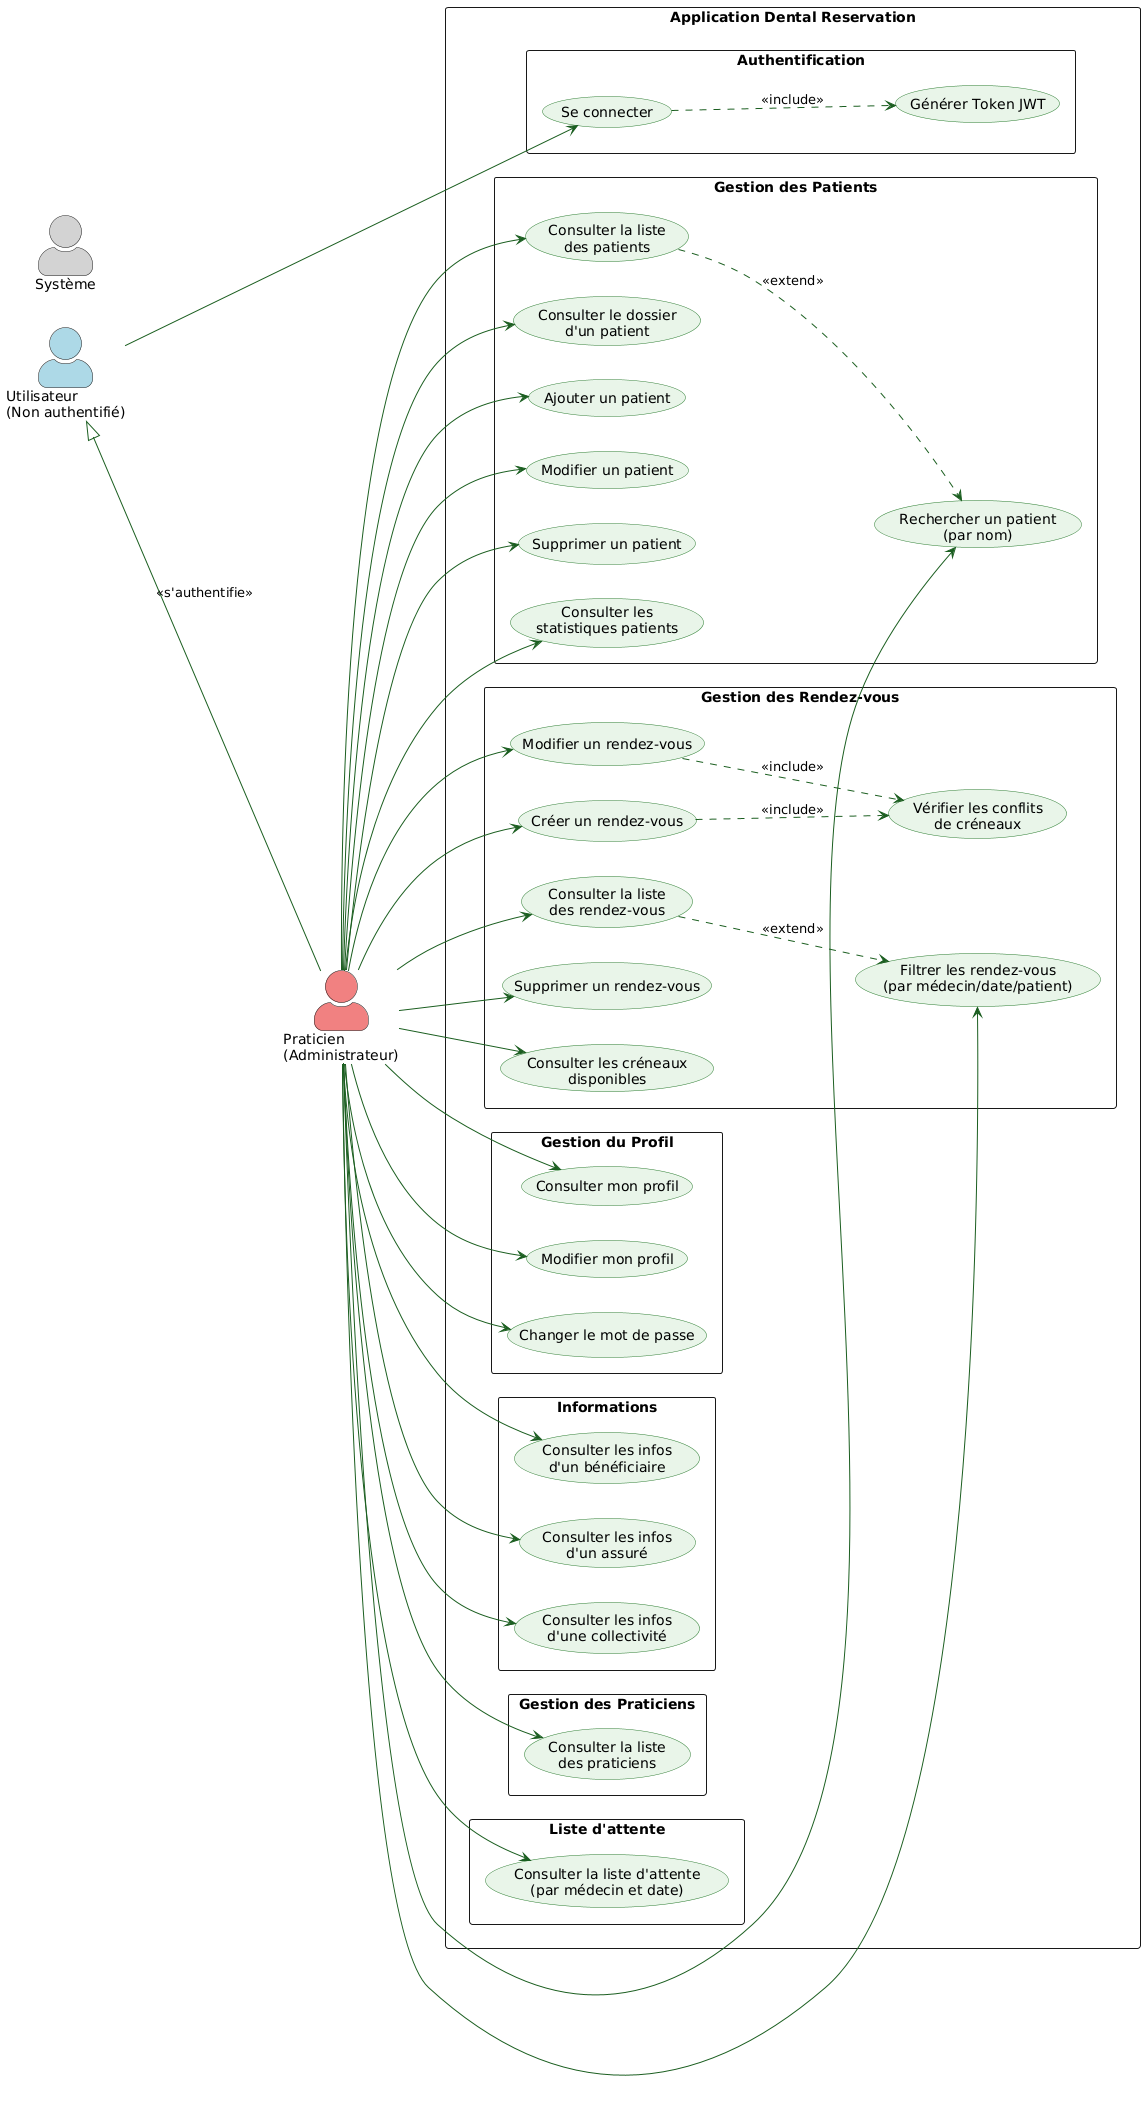
\includegraphics[width=0.75\textwidth]{use_case_diagram.png}
\end{figure}
\begin{figure}[H]
%\fbox{\parbox{0.85\textwidth}{\centering\vspace{2cm}\textit{Diagramme de cas d'utilisation}\\\texttt{diagrams/use\_case\_diagram.puml}\vspace{2cm}}}
\caption{Diagramme de cas d'utilisation}
\label{fig:use_case}
\end{figure}

\subsection{Acteurs}
\begin{itemize}
    \item \textbf{Utilisateur non authentifié (Guest)}~: ne peut accéder qu'à la page de connexion.
    \item \textbf{Praticien (Administrateur)}~: après authentification, a accès à l'ensemble des fonctionnalités.
\end{itemize}

\subsection{Packages de cas d'utilisation}

\begin{enumerate}
    \item \textbf{Authentification} --- Se connecter~; Générer Token JWT (\texttt{<<include>>})
    \item \textbf{Gestion des Patients} --- Consulter la liste~; Rechercher~; Consulter le dossier~; Ajouter~; Modifier~; Supprimer~; Statistiques
    \item \textbf{Gestion des Rendez-vous} --- Consulter la liste~; Créer (inclut \emph{Vérifier les conflits})~; Modifier~; Supprimer~; Créneaux disponibles~; Filtrer
    \item \textbf{Gestion du Profil} --- Consulter~; Modifier~; Changer le mot de passe
    \item \textbf{Informations} --- Bénéficiaire~; Assuré~; Collectivité
    \item \textbf{Gestion des Praticiens} --- Consulter la liste
    \item \textbf{Liste d'attente} --- Consulter par médecin et date
\end{enumerate}

% ============================================================
\section{Diagramme de Classes}

Le diagramme de classes (Figure~\ref{fig:class_diagram}) modélise l'ensemble des entités du système, leurs attributs, leurs méthodes et les relations entre elles.

\begin{figure}[H]
\centering
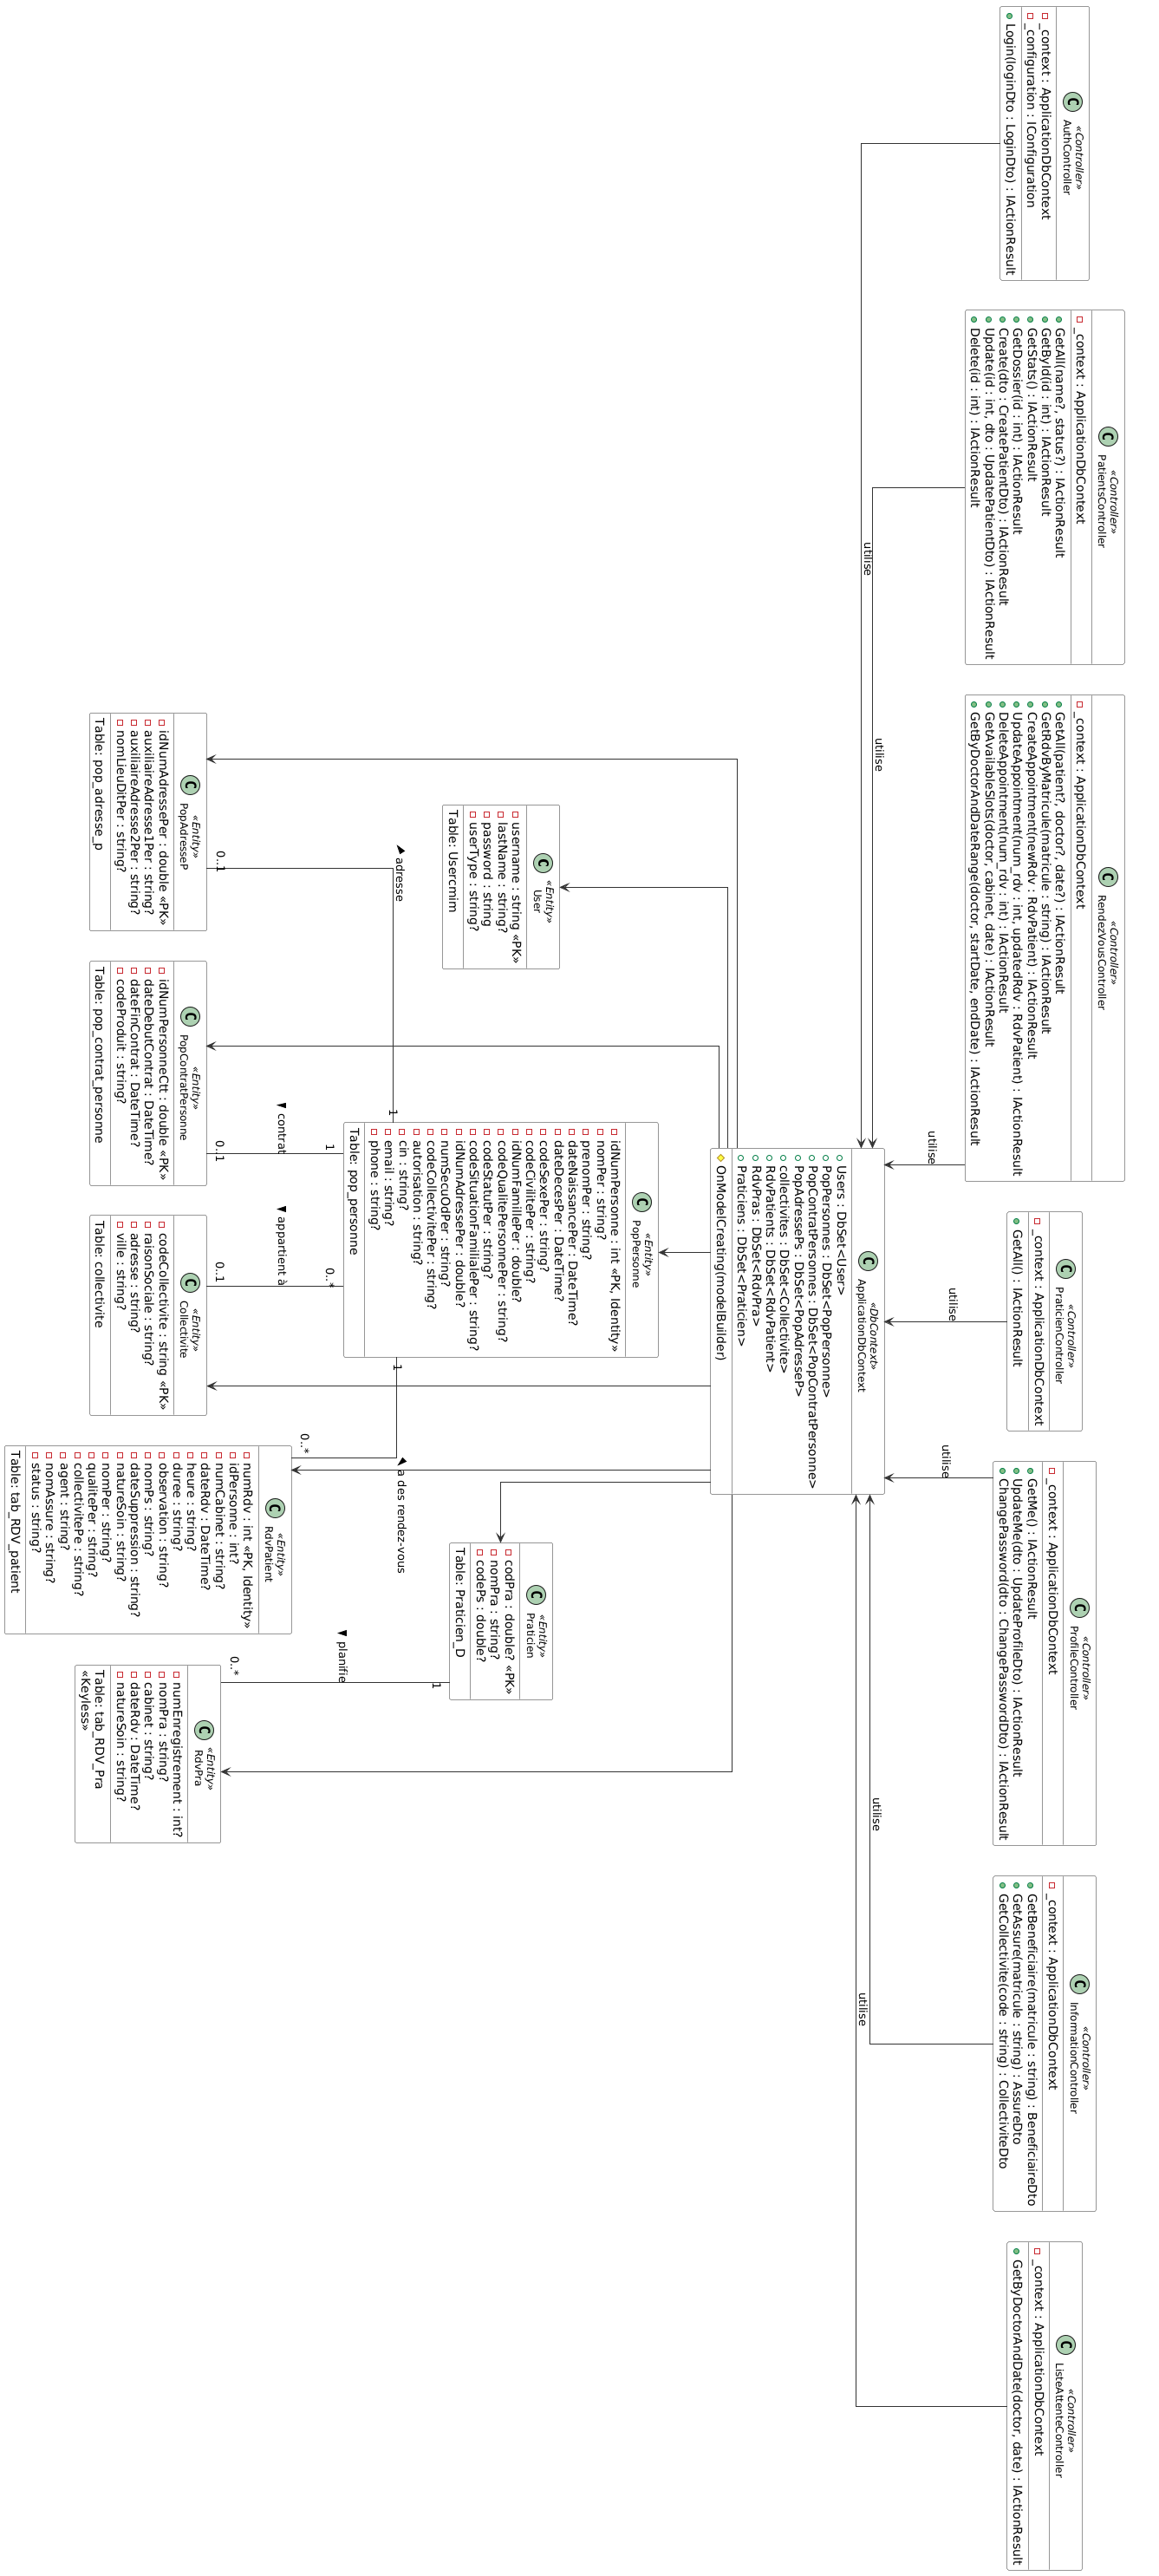
\includegraphics[width=0.70\textwidth]{class_diagram1.png}
%\fbox{\parbox{0.85\textwidth}{\centering\vspace{2cm}\textit{Diagramme de classes}\\\texttt{diagrams/class_diagram.puml}\vspace{2cm}}}
\caption{Diagramme de classes}
\label{fig:class_diagram}
\end{figure}

\subsection{Entités (mapping base de données)}

\begin{itemize}
    \item \textbf{User} $\rightarrow$ table \texttt{Usercmim}\\
    Attributs~: \texttt{username} (PK), \texttt{lastName}, \texttt{password}, \texttt{userType}\\
    Rôle~: stocke les identifiants des praticiens

    \item \textbf{PopPersonne} $\rightarrow$ table \texttt{pop\_personne}\\
    Attributs~: \texttt{IdNumPersonne} (PK, auto), \texttt{NomPer}, \texttt{PrenomPer}, \texttt{DteNaisPer}, \texttt{SexePer}, \texttt{CIN}, \texttt{NumSecuOdPer} (matricule), \texttt{CodeCollectivite}, \texttt{Email}, \texttt{Phone}\\
    Rôle~: entité centrale représentant un patient

    \item \textbf{PopAdresseP} $\rightarrow$ table \texttt{pop\_adresse\_p}\\
    Attributs~: \texttt{IdNumAdressePer} (PK), \texttt{LibAdresse}\\
    Rôle~: adresse postale du patient

    \item \textbf{PopContratPersonne} $\rightarrow$ table \texttt{pop\_contrat\_personne}\\
    Attribut~: \texttt{IdNumPersonneCtt} (PK)\\
    Rôle~: contrat d'assurance

    \item \textbf{Collectivite} $\rightarrow$ table \texttt{collectivite}\\
    Attributs~: \texttt{CodeCollectivite} (PK), \texttt{RaisonSociale}, \texttt{Adresse}, \texttt{Ville}, \texttt{Region}\\
    Rôle~: organisme d'appartenance

    \item \textbf{RdvPatient} $\rightarrow$ table \texttt{tab\_RDV\_patient}\\
    Attributs~: \texttt{NumRdv} (PK, auto), \texttt{IdPersonne} (FK), \texttt{DateRdv}, \texttt{Heure}, \texttt{DureeRdv}, \texttt{NomPs}, \texttt{Cabinet}, \texttt{NatureSoin}, \texttt{Status}, \texttt{Notes}\\
    Rôle~: rendez-vous patient

    \item \textbf{RdvPra} $\rightarrow$ table \texttt{tab\_RDV\_Pra} (Keyless)\\
    Attributs~: \texttt{DateRDV}, \texttt{HeureDebut}, \texttt{HeureFin}, \texttt{NomPra}, \texttt{IdRDV}\\
    Rôle~: planification praticien

    \item \textbf{Praticien} $\rightarrow$ table \texttt{Praticien\_D}\\
    Attributs~: \texttt{CodPra} (PK), \texttt{NomPra}, \texttt{CodePs}\\
    Rôle~: référentiel praticiens
\end{itemize}

\subsection{DTOs (Data Transfer Objects)}

\begin{itemize}
    \item \textbf{LoginDto}~: \texttt{username}, \texttt{password}
    \item \textbf{PatientDto}~: \texttt{nom}, \texttt{prenom}, \texttt{dateNaissance}, \texttt{sexe}, \texttt{cin}, \texttt{matricule}, etc.
    \item \textbf{AssureDto}~: informations de l'assuré (personne, adresse, contrat)
    \item \textbf{BeneficiaireDto}~: informations du bénéficiaire
    \item \textbf{CollectiviteDto}~: informations de la collectivité
\end{itemize}

\subsection{Relations entre les classes}

\begin{itemize}
    \item \texttt{PopPersonne} \textbf{1 --- 0..1} \texttt{PopAdresseP}~: chaque patient peut avoir une adresse
    \item \texttt{PopPersonne} \textbf{1 --- 0..1} \texttt{PopContratPersonne}~: contrat d'assurance
    \item \texttt{PopPersonne} \textbf{0..* --- 0..1} \texttt{Collectivite}~: appartenance à une collectivité
    \item \texttt{PopPersonne} \textbf{1 --- 0..*} \texttt{RdvPatient}~: un patient a zéro ou plusieurs rendez-vous
    \item \texttt{Praticien} \textbf{1 --- 0..*} \texttt{RdvPra}~: planifications du praticien
    \item Tous les contrôleurs dépendent de \texttt{ApplicationDbContext} (injection de dépendance)
\end{itemize}

% ============================================================
\section{Diagrammes de Séquence}

Trois diagrammes de séquence décrivent les interactions entre les composants principaux du système.

\subsection{Séquence d'authentification}

\begin{figure}[H]
\centering
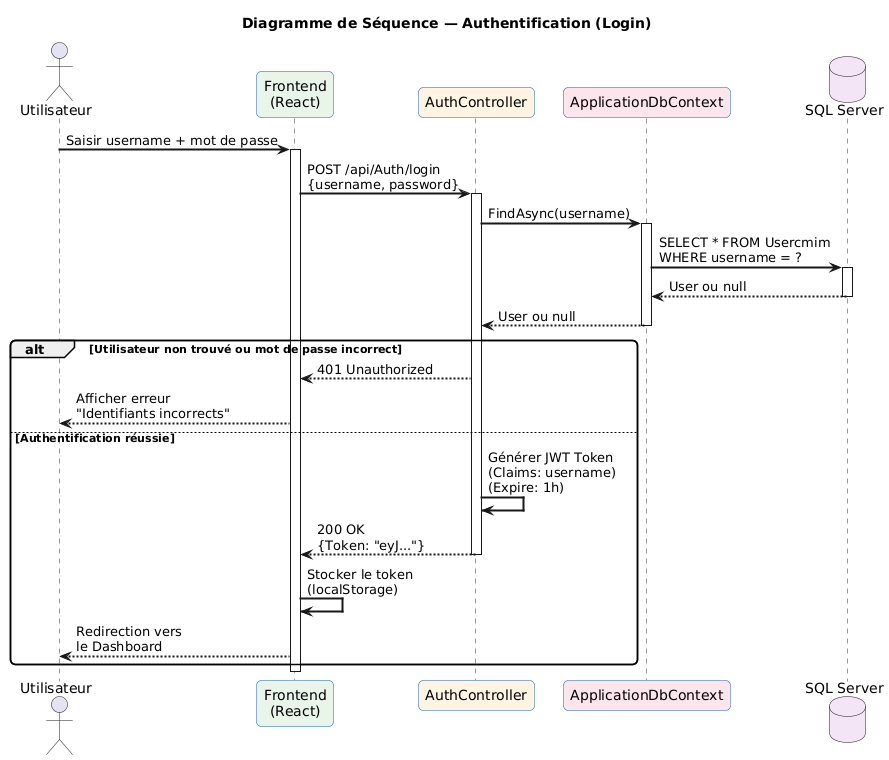
\includegraphics[width=0.9\textwidth]{sequence_authentification.png}
%\fbox{\parbox{0.85\textwidth}{\centering\vspace{2cm}\textit{Diagramme de séquence --- Authentification}\\\texttt{diagrams/sequence\_authentification.puml}\vspace{2cm}}}
\caption{Diagramme de séquence~: Authentification}
\label{fig:seq_auth}
\end{figure}

Le flux d'authentification implique quatre participants~: \textbf{Utilisateur}, \textbf{Frontend React}, \textbf{AuthController} et \textbf{Base de données SQL Server}.

\subsubsection{Scénario nominal (succès)}
\begin{enumerate}
    \item L'utilisateur saisit son email et son mot de passe sur la page Login.
    \item Le composant \texttt{Login.tsx} appelle \texttt{apiService.login(email, password)}.
    \item Le service API envoie \texttt{POST /api/Auth/login} avec \texttt{\{username, password\}}.
    \item Le \texttt{AuthController} recherche l'utilisateur via LINQ~: \texttt{dbContext.Users.FirstOrDefault(...)}.
    \item Comparaison du mot de passe.
    \item Création du \texttt{JwtSecurityToken} avec claim \texttt{username}, expiration 1h, signature HMAC-SHA256.
    \item Retour du token dans la réponse \texttt{200 OK}.
    \item Stockage dans \texttt{localStorage} et redirection vers \texttt{/dashboard}.
\end{enumerate}

\subsubsection{Scénario alternatif (échec)}
Si l'utilisateur n'existe pas ou si le mot de passe est incorrect~: réponse \texttt{401 Unauthorized}. Le frontend affiche une notification toast rouge.

\subsection{Séquence de gestion des rendez-vous}

\begin{figure}[H]
\centering
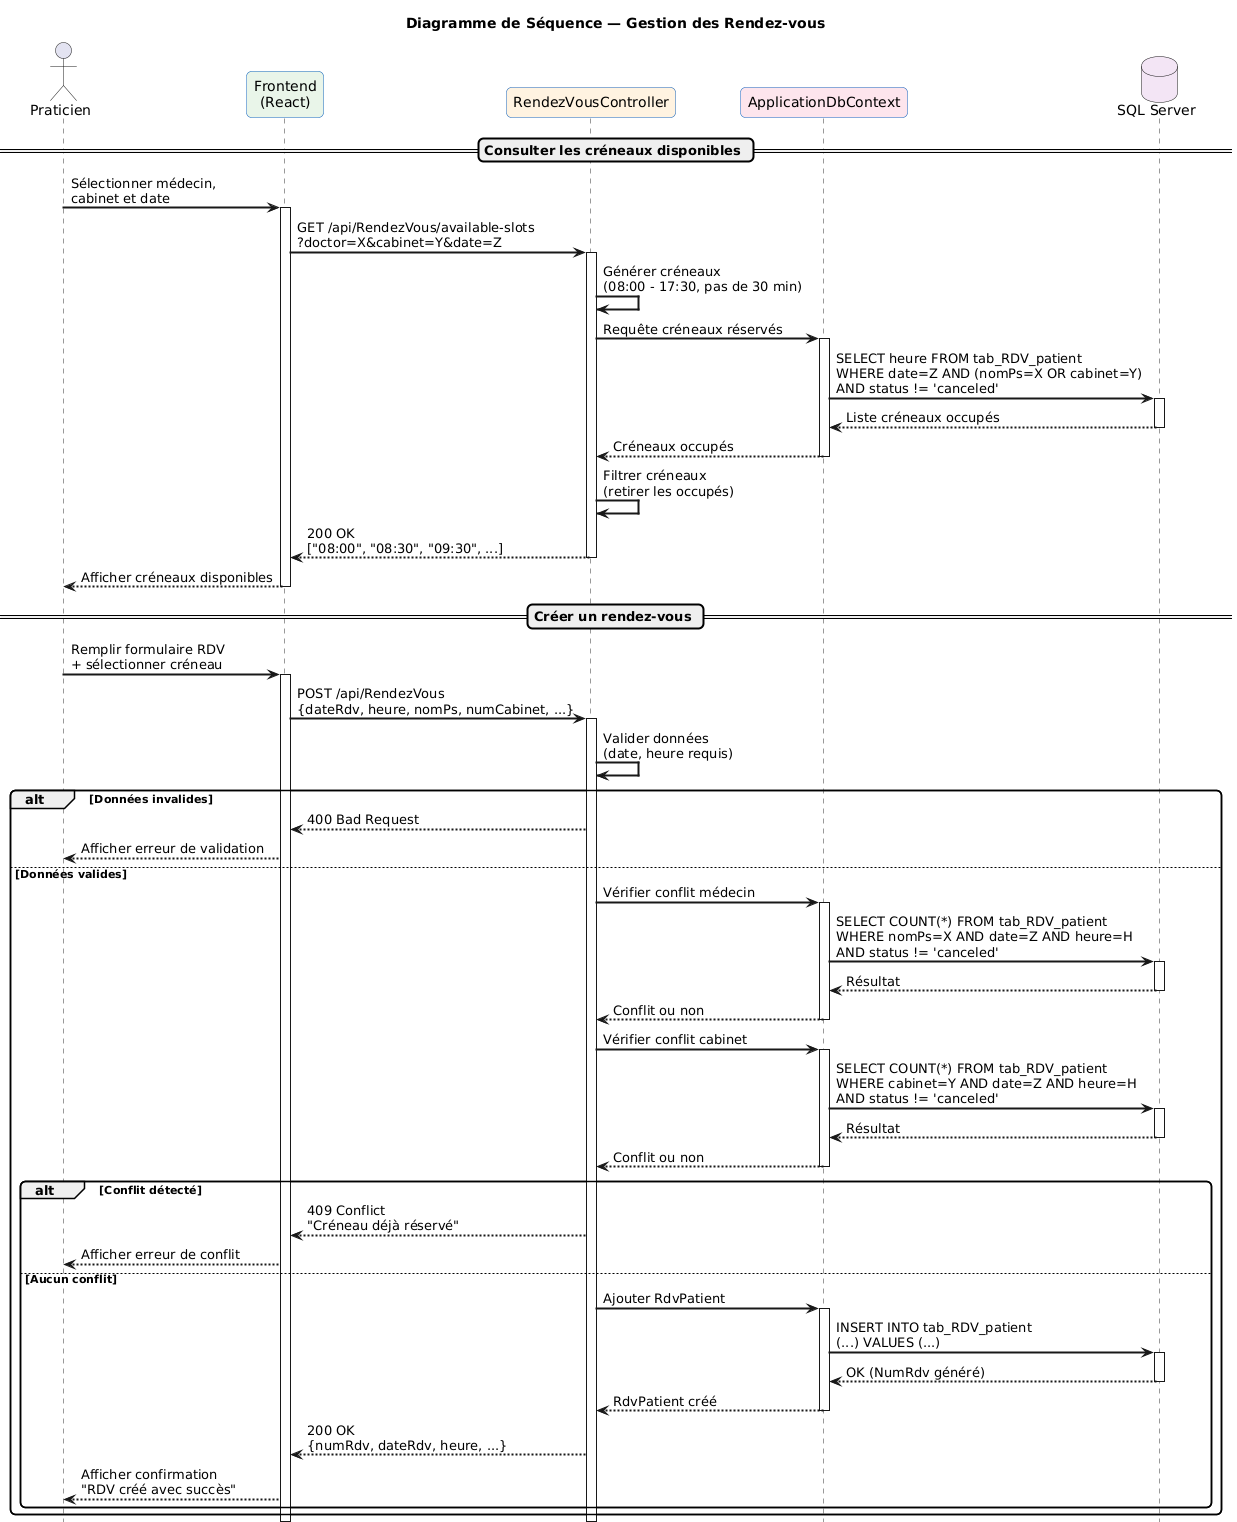
\includegraphics[width=0.9\textwidth]{sequence_rendez_vous1.png}
\end{figure}
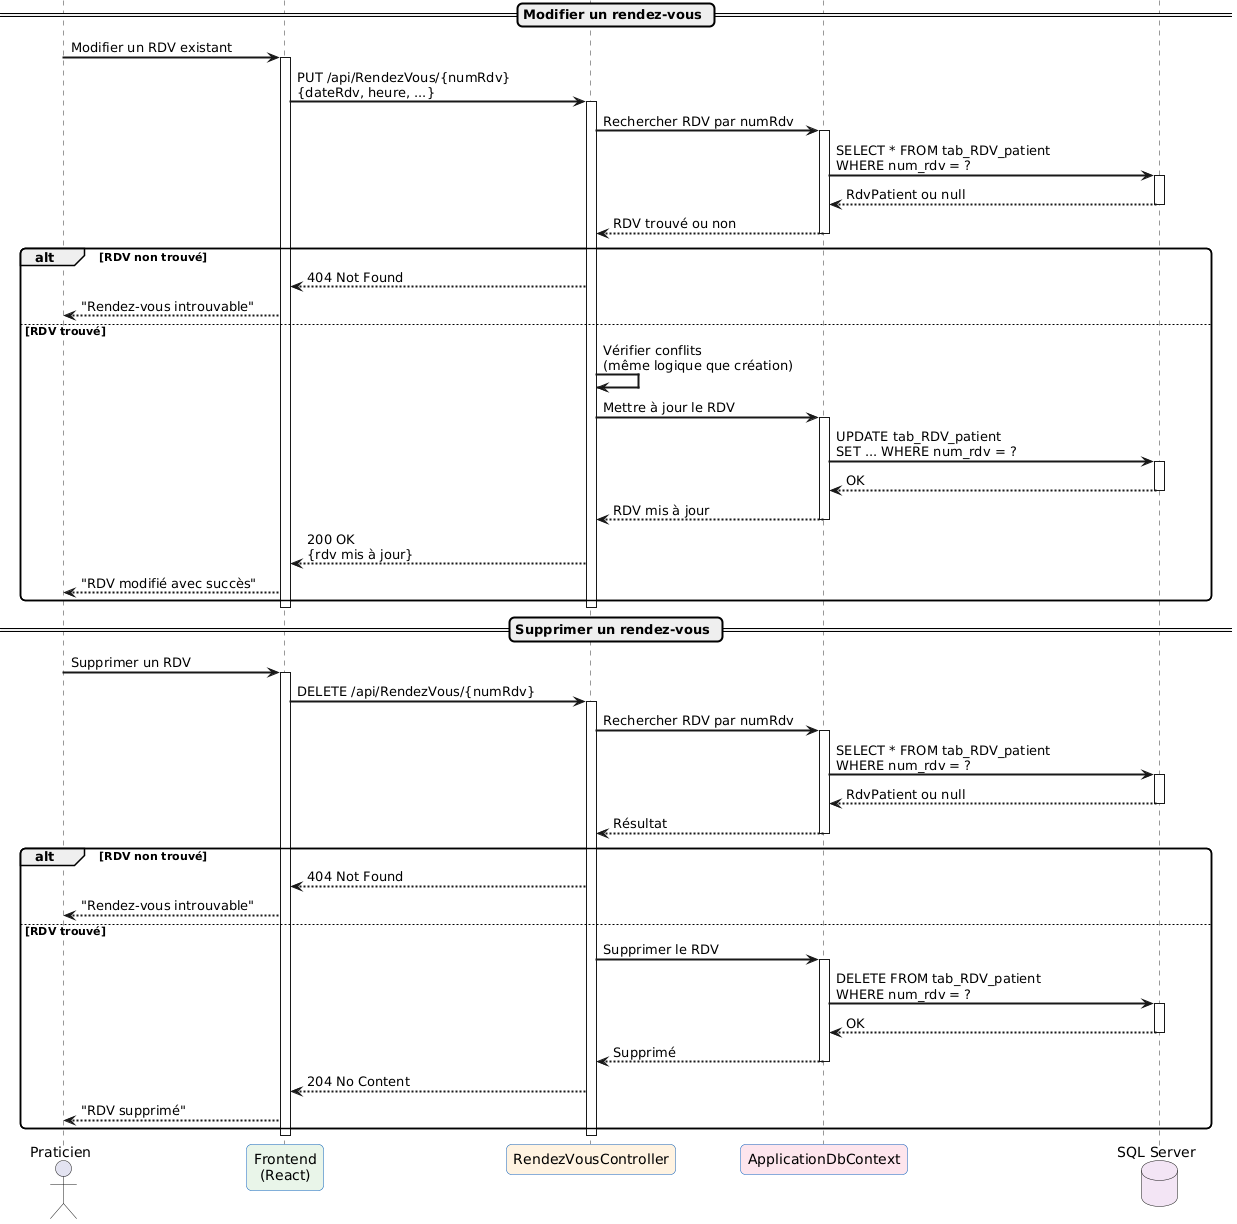
\includegraphics[width=0.9\textwidth]{sequence_rendez_vous2.png}
\begin{figure}[H]
%\fbox{\parbox{0.85\textwidth}{\centering\vspace{2cm}\textit{Diagramme de séquence --- Gestion des rendez-vous}\\\texttt{diagrams/sequence\_rendez\_vous.puml}\vspace{2cm}}}
\caption{Diagramme de séquence~: Gestion des rendez-vous}
\label{fig:seq_rdv}
\end{figure}

Ce diagramme couvre quatre opérations~:

\begin{enumerate}
    \item \textbf{Consulter les créneaux disponibles}~: génération de la grille 08:00--17:30, soustraction des créneaux réservés.
    \item \textbf{Créer un rendez-vous}~: validation $\rightarrow$ vérification conflit médecin $\rightarrow$ vérification conflit cabinet $\rightarrow$ insertion avec statut \og pending \fg.
    \item \textbf{Modifier un rendez-vous}~: même logique de conflits $\rightarrow$ mise à jour.
    \item \textbf{Supprimer un rendez-vous}~: confirmation $\rightarrow$ suppression $\rightarrow$ \texttt{204 No Content}.
\end{enumerate}

\subsection{Séquence de gestion des patients}

\begin{figure}[H]
\centering
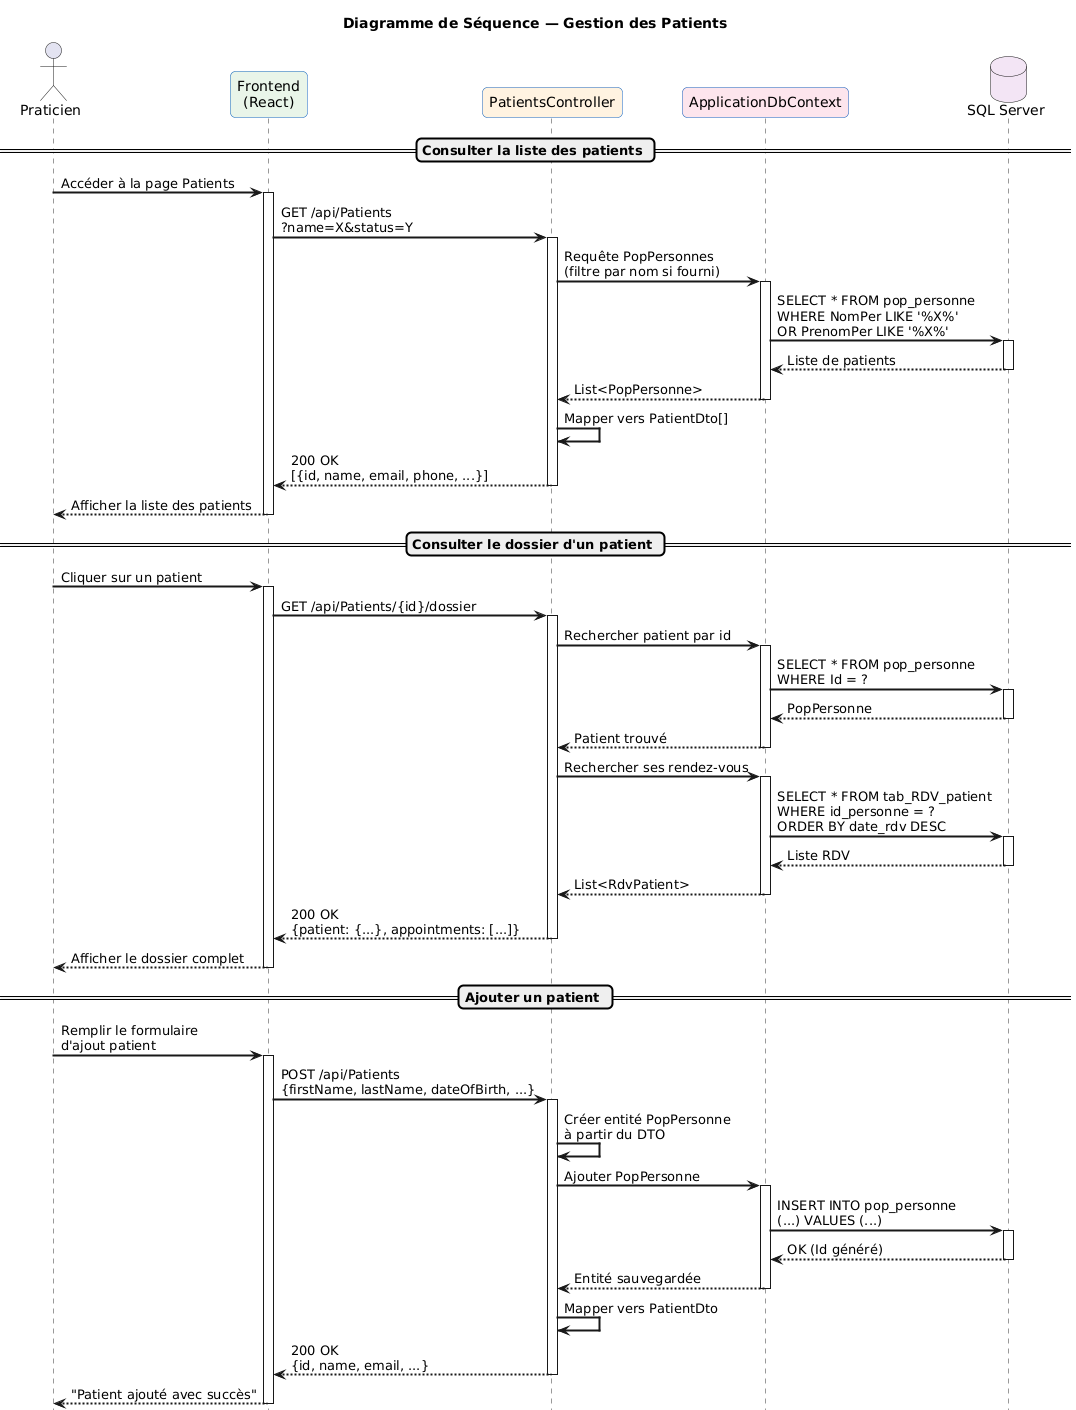
\includegraphics[width=0.9\textwidth]{sequence_patients1.png}
\end{figure}
\begin{figure}[H]
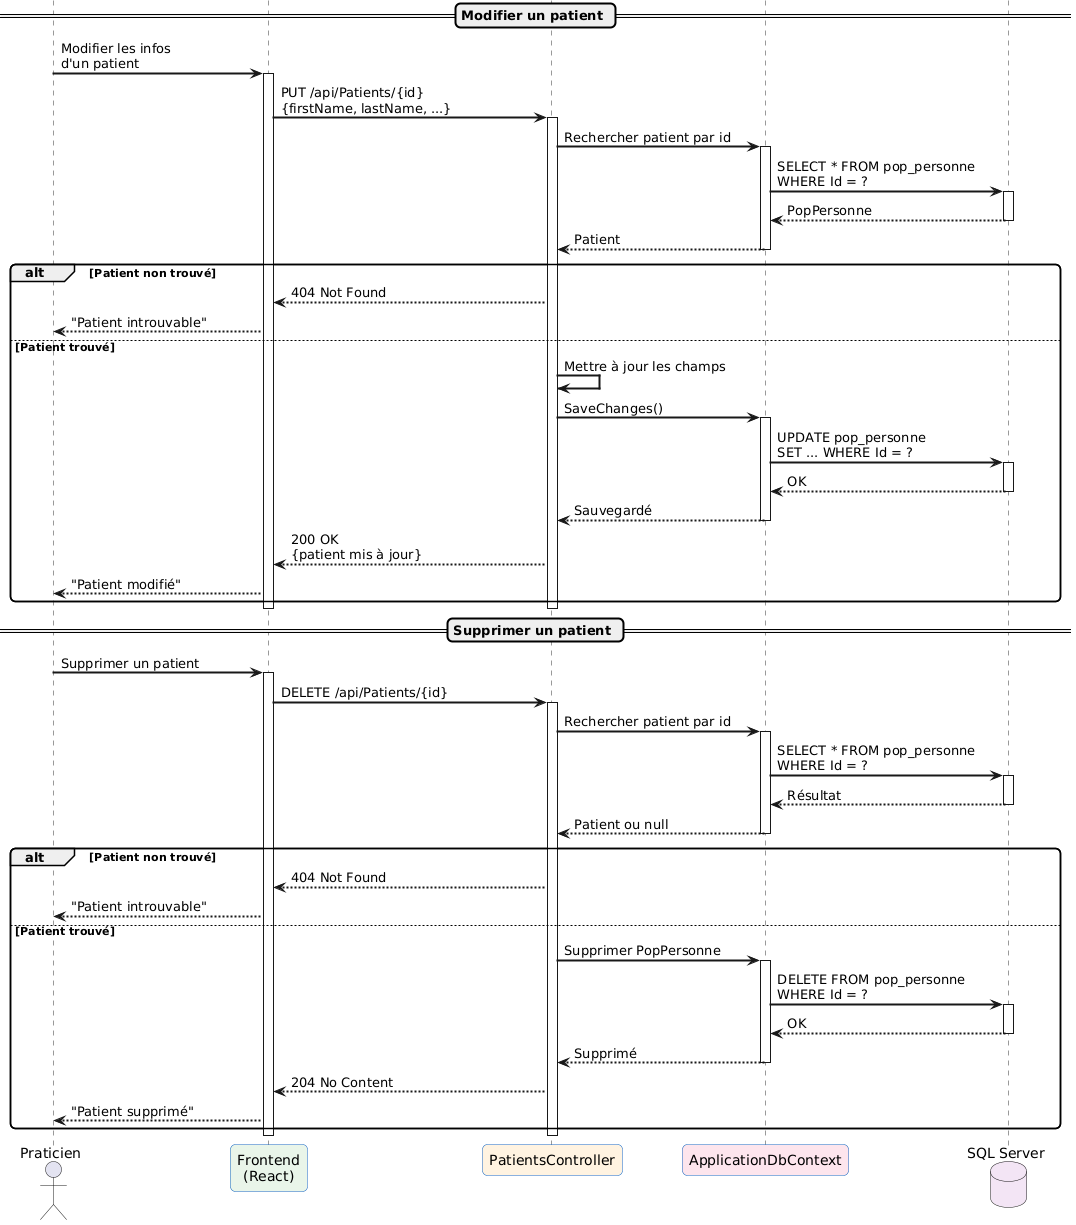
\includegraphics[width=0.9\textwidth]{sequence_patients2.png}
%\fbox{\parbox{0.85\textwidth}{\centering\vspace{2cm}\textit{Diagramme de séquence --- Gestion des patients}\\\texttt{diagrams/sequence\_patients.puml}\vspace{2cm}}}
\caption{Diagramme de séquence~: Gestion des patients}
\label{fig:seq_patients}
\end{figure}

Opérations CRUD complètes sur \texttt{PopPersonne}~:

\begin{enumerate}
    \item \textbf{Consulter la liste}~: filtre optionnel $\rightarrow$ mapping \texttt{PopPersonne} $\rightarrow$ \texttt{PatientDto} avec calcul du genre.
    \item \textbf{Consulter le dossier}~: patient + rendez-vous triés par date décroissante.
    \item \textbf{Ajouter}~: formulaire 16 champs $\rightarrow$ création \texttt{PopPersonne} $\rightarrow$ retour DTO.
    \item \textbf{Modifier}~: mise à jour partielle des champs non-null.
    \item \textbf{Supprimer}~: suppression $\rightarrow$ \texttt{204 No Content}.
\end{enumerate}

% ============================================================
\section{Diagrammes d'Activité}

\subsection{Activité d'authentification}

\begin{figure}[H]
\centering
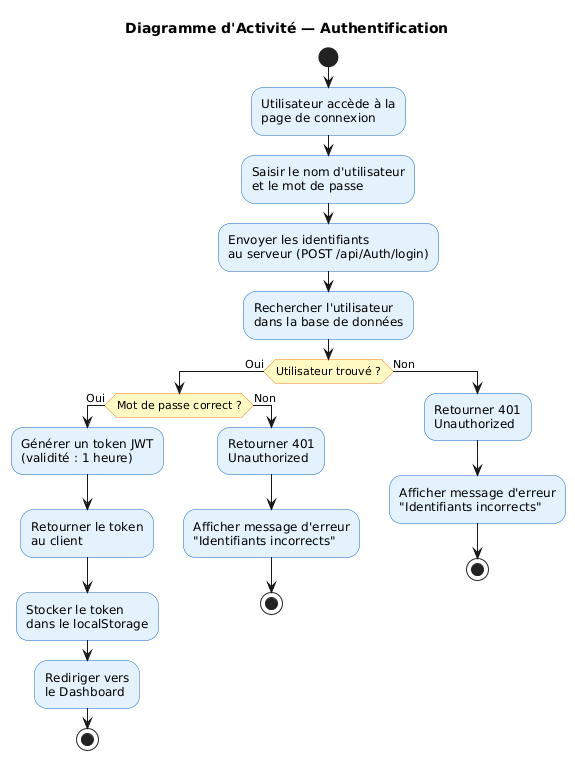
\includegraphics[width=0.7\textwidth]{activity_authentification.png}
%\fbox{\parbox{0.85\textwidth}{\centering\vspace{2cm}\textit{Diagramme d'activité --- Authentification}\\\texttt{diagrams/activity\_authentification.puml}\vspace{2cm}}}
\caption{Diagramme d'activité~: Authentification}
\label{fig:act_auth}
\end{figure}

Le flux décisionnel~: saisie des identifiants $\rightarrow$ recherche en BDD $\rightarrow$ vérification du mot de passe $\rightarrow$ si OK~: génération JWT + stockage + redirection~; si KO~: affichage erreur.

\subsection{Activité de création d'un rendez-vous}

\begin{figure}[H]
\centering
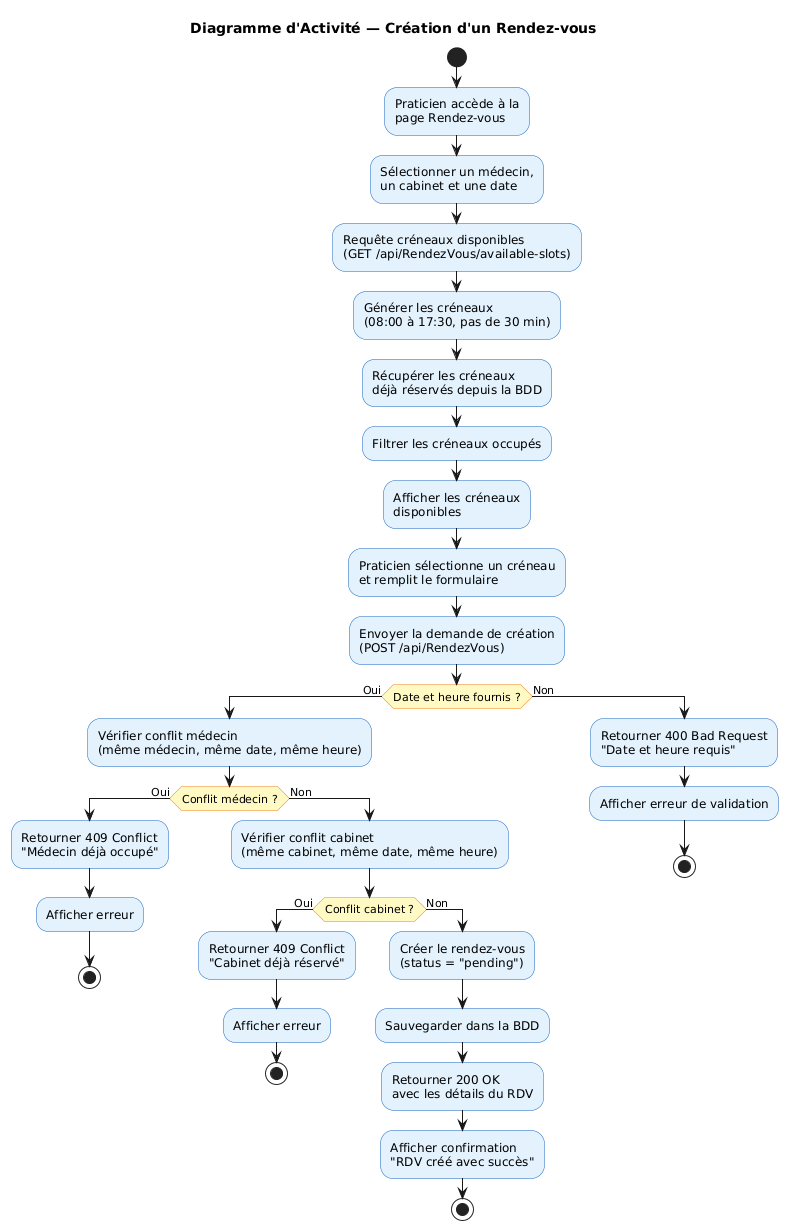
\includegraphics[width=0.7\textwidth]{activity_rendez_vous.png}
%\fbox{\parbox{0.85\textwidth}{\centering\vspace{2cm}\textit{Diagramme d'activité --- Création d'un rendez-vous}\\\texttt{diagrams/activity\_rendez\_vous.puml}\vspace{2cm}}}
\caption{Diagramme d'activité~: Création d'un rendez-vous}
\label{fig:act_rdv}
\end{figure}

Flux~: sélection patient/médecin/cabinet $\rightarrow$ vérification date et heure $\rightarrow$ vérification conflit médecin $\rightarrow$ vérification conflit cabinet $\rightarrow$ si aucun conflit~: insertion avec statut \og pending \fg~; sinon~: erreur 409.

\subsection{Activité de gestion des patients (CRUD)}

\begin{figure}[H]
\centering
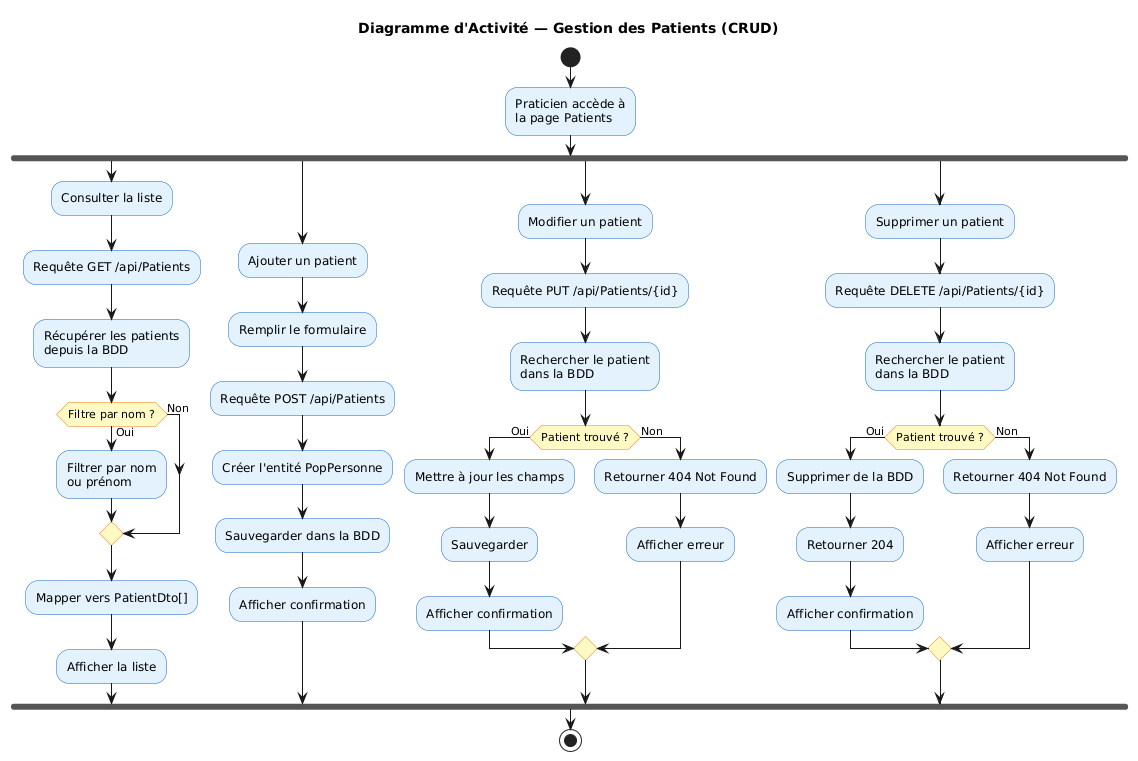
\includegraphics[width=0.7\textwidth]{activity_patients.png}
%\fbox{\parbox{0.85\textwidth}{\centering\vspace{2cm}\textit{Diagramme d'activité --- Gestion des patients}\\\texttt{diagrams/activity\_patients.puml}\vspace{2cm}}}
\caption{Diagramme d'activité~: Gestion des patients (CRUD)}
\label{fig:act_patients}
\end{figure}

Quatre opérations en parallèle (fork/join)~:
\begin{itemize}
    \item \textbf{Consulter}~: charger la liste $\rightarrow$ appliquer filtres $\rightarrow$ afficher tableau
    \item \textbf{Ajouter}~: ouvrir modale $\rightarrow$ remplir formulaire $\rightarrow$ POST $\rightarrow$ rafraîchir
    \item \textbf{Modifier}~: sélectionner $\rightarrow$ ouvrir modale $\rightarrow$ PUT $\rightarrow$ rafraîchir
    \item \textbf{Supprimer}~: sélectionner $\rightarrow$ confirmer $\rightarrow$ DELETE $\rightarrow$ rafraîchir
\end{itemize}

\section{Conclusion}

Ce chapitre a présenté la conception UML complète de l'application \textbf{Dental Reservation} à travers 8 diagrammes couvrant les cas d'utilisation, les classes, les séquences d'interaction et les flux d'activité. Cette modélisation a servi de base solide pour la phase de réalisation détaillée dans le chapitre suivant.

% ============================================================
%  Chapitre 4 : Réalisation
% ============================================================

% ---- Page de titre du chapitre ----
\clearpage
\thispagestyle{chaptertitlepage}
\vspace*{\fill}
\begin{center}
\rule{\textwidth}{0.4pt}\\[0.8cm]
{\fontsize{24}{29}\selectfont\bfseries Chapitre 4}\\[0.6cm]
{\fontsize{18}{22}\selectfont Réalisation}\\[0.8cm]
\rule{\textwidth}{0.4pt}
\end{center}
\vspace*{\fill}
\clearpage

% ---- Contenu du chapitre ----
\chapter{Réalisation}

\section{Introduction}

La phase de réalisation a consisté à implémenter l'ensemble des fonctionnalités spécifiées dans l'étude fonctionnelle et technique, et modélisées dans les diagrammes UML. Le développement a suivi une approche itérative, en commençant par la couche backend (API et base de données), puis la couche frontend (interface utilisateur).

L'environnement de développement comprend~:
\begin{itemize}
    \item \textbf{IDE}~: Visual Studio Code avec les extensions C\#, TypeScript, Tailwind CSS IntelliSense
    \item \textbf{Backend}~: \texttt{dotnet run} (port HTTPS 7091, HTTP 5057)
    \item \textbf{Frontend}~: \texttt{npm run dev} (port 8080, proxy vers le backend)
    \item \textbf{Base de données}~: SQL Server LocalDB (\texttt{(localdb)\textbackslash MSSQLLocalDB}, base \texttt{CabinetD})
\end{itemize}

% ============================================================
\section{Sécurité~: Authentification et Contrôle d'accès}

La sécurité de l'application repose sur le standard \textbf{JSON Web Token (JWT)}, un mécanisme d'authentification \emph{stateless} largement adopté dans les architectures REST modernes.

\subsection{Configuration JWT côté backend}

Dans le fichier \texttt{Program.cs}, le middleware d'authentification ASP.NET Core est configuré au démarrage~:

\begin{lstlisting}[language={[Sharp]C}, caption={Configuration JWT dans Program.cs}]
builder.Services.AddAuthentication(JwtBearerDefaults.AuthenticationScheme)
    .AddJwtBearer(options => {
        options.TokenValidationParameters = new TokenValidationParameters {
            ValidateIssuer = true,
            ValidateAudience = true,
            ValidateLifetime = true,
            ValidateIssuerSigningKey = true,
            ValidIssuer = configuration["Jwt:Issuer"],
            ValidAudience = configuration["Jwt:Audience"],
            IssuerSigningKey = new SymmetricSecurityKey(
                Encoding.UTF8.GetBytes(configuration["Jwt:Key"]))
        };
    });
\end{lstlisting}

Les paramètres JWT sont stockés dans \texttt{appsettings.json}~:
\begin{itemize}
    \item \texttt{Jwt:Key}~: clé secrète HMAC-SHA256 pour la signature du token
    \item \texttt{Jwt:Issuer}~: identifiant de l'émetteur (le backend)
    \item \texttt{Jwt:Audience}~: identifiant de l'audience (le frontend)
\end{itemize}

Le \texttt{AuthController} expose un unique endpoint \texttt{POST /api/Auth/login} qui~:
\begin{enumerate}
    \item Reçoit un \texttt{LoginDto} contenant \texttt{username} et \texttt{password}.
    \item Recherche l'utilisateur dans la table \texttt{Usercmim} par \texttt{username}.
    \item Compare le mot de passe fourni avec celui stocké en base.
    \item Si valide, crée un \texttt{SecurityTokenDescriptor} avec un claim \texttt{ClaimTypes.Name}, une expiration de 1 heure, et une signature HMAC-SHA256.
    \item Retourne le token JWT sérialisé et les informations utilisateur.
\end{enumerate}

\subsection{Protection côté frontend}

Le frontend utilise un \textbf{pattern Provider/Context} (React Context API) pour gérer l'authentification de manière globale~:

\begin{itemize}
    \item \textbf{AuthProvider} (\texttt{use-auth.tsx})~: enveloppe toute l'application et expose via le contexte~:
    \begin{itemize}
        \item \texttt{user}~: l'utilisateur connecté (ou null)
        \item \texttt{isAuthenticated}~: booléen dérivé de la présence du token
        \item \texttt{login(email, password)}~: appelle l'API, stocke le token dans \texttt{localStorage}
        \item \texttt{logout()}~: supprime le token, redirige vers la page de connexion
        \item \texttt{updateUser(userData)}~: met à jour les données utilisateur locales
    \end{itemize}
    
    \item \textbf{ProtectedRoute}~: composant wrapper qui vérifie \texttt{isAuthenticated}. Si l'utilisateur n'est pas connecté, redirection automatique vers \texttt{/}.
    
    \item \textbf{ApiService.getAuthHeaders()}~: méthode qui injecte automatiquement l'en-tête \texttt{Authorization: Bearer <token>} dans chaque requête API.
\end{itemize}

\subsection{Swagger avec authentification}

En environnement de développement, Swagger UI est activé avec un bouton \og Authorize \fg{} permettant de saisir le token JWT. La configuration inclut un \texttt{SecurityDefinition} de type Bearer et un \texttt{SecurityRequirement} global, permettant de tester tous les endpoints protégés directement depuis le navigateur.

% ============================================================
\section{Gestion des requêtes et communication client-serveur}

\subsection{Service API centralisé}

Toute la communication entre le frontend et le backend est centralisée dans la classe \textbf{ApiService} (\texttt{src/lib/api.ts}). Cette classe fournit une abstraction de haut niveau sur l'API Fetch~:

\begin{itemize}
    \item \textbf{Authentification}~: \texttt{login()}, \texttt{logout()}, \texttt{isAuthenticated()}, \texttt{getToken()}, \texttt{getAuthHeaders()}
    \item \textbf{Patients}~: \texttt{getPatients()}, \texttt{createPatient()}, \texttt{updatePatient()}, \texttt{deletePatient()}, \texttt{getPatientStats()}, \texttt{getPatientDossier()}
    \item \textbf{Rendez-vous}~: \texttt{getAppointments()}, \texttt{createAppointment()}, \texttt{updateAppointment()}, \texttt{deleteAppointment()}, \texttt{getAvailableSlots()}
    \item \textbf{Profil}~: \texttt{getProfile()}, \texttt{updateProfile()}, \texttt{changePassword()}
\end{itemize}

Chaque méthode gère automatiquement l'injection des headers d'authentification, le \texttt{Content-Type: application/json}, le parsing JSON et la gestion d'erreurs.

\subsection{Gestion du cache avec React Query}

Le frontend utilise \textbf{TanStack React Query} pour optimiser les interactions avec l'API~:

\begin{itemize}
    \item \textbf{Queries} (\texttt{useQuery})~: les données sont mises en cache avec des clés uniques (ex~: \texttt{["patients"]}, \texttt{["appointments"]}). Le cache évite les requêtes réseau redondantes.
    \item \textbf{Mutations} (\texttt{useMutation})~: les opérations d'écriture invalident automatiquement les caches associés via \texttt{queryClient.invalidateQueries()} après succès, déclenchent des notifications toast et gèrent les états de chargement.
\end{itemize}

\subsection{Détection des conflits de rendez-vous}

La détection des conflits est implémentée côté serveur dans le \texttt{RendezVousController}~:

\begin{itemize}
    \item \textbf{Conflit médecin}~: vérifie qu'aucun rendez-vous actif (statut $\neq$ \og canceled \fg) n'existe pour le même médecin, à la même date et heure. Si conflit $\rightarrow$ \texttt{409 Conflict}.
    \item \textbf{Conflit cabinet}~: vérifie qu'aucun rendez-vous actif n'existe pour le même cabinet, à la même date et heure. Si conflit $\rightarrow$ \texttt{409 Conflict}.
\end{itemize}

Cette double vérification garantit qu'un médecin ne peut pas avoir deux consultations simultanées et qu'un cabinet ne peut pas être utilisé par deux médecins en même temps.

% ============================================================
\section{Notifications et retour utilisateur}

L'application implémente un système de notifications visuelles basé sur les composants \textbf{Toast} de shadcn/ui~:

\begin{itemize}
    \item \textbf{Notifications toast}~: chaque action déclenche une notification éphémère (vert = succès, rouge = erreur, bleu = information).
    \item \textbf{Panneau de notifications} (\texttt{NotificationsPanel.tsx})~: accessible via l'icône cloche dans la barre de navigation, il affiche l'historique avec horodatage relatif et un badge de compteur.
\end{itemize}

% ============================================================
\section{Interface d'administration --- Pages de l'application}

\subsection{Page de connexion (Login)}

 \begin{figure}[H]
 \centering
 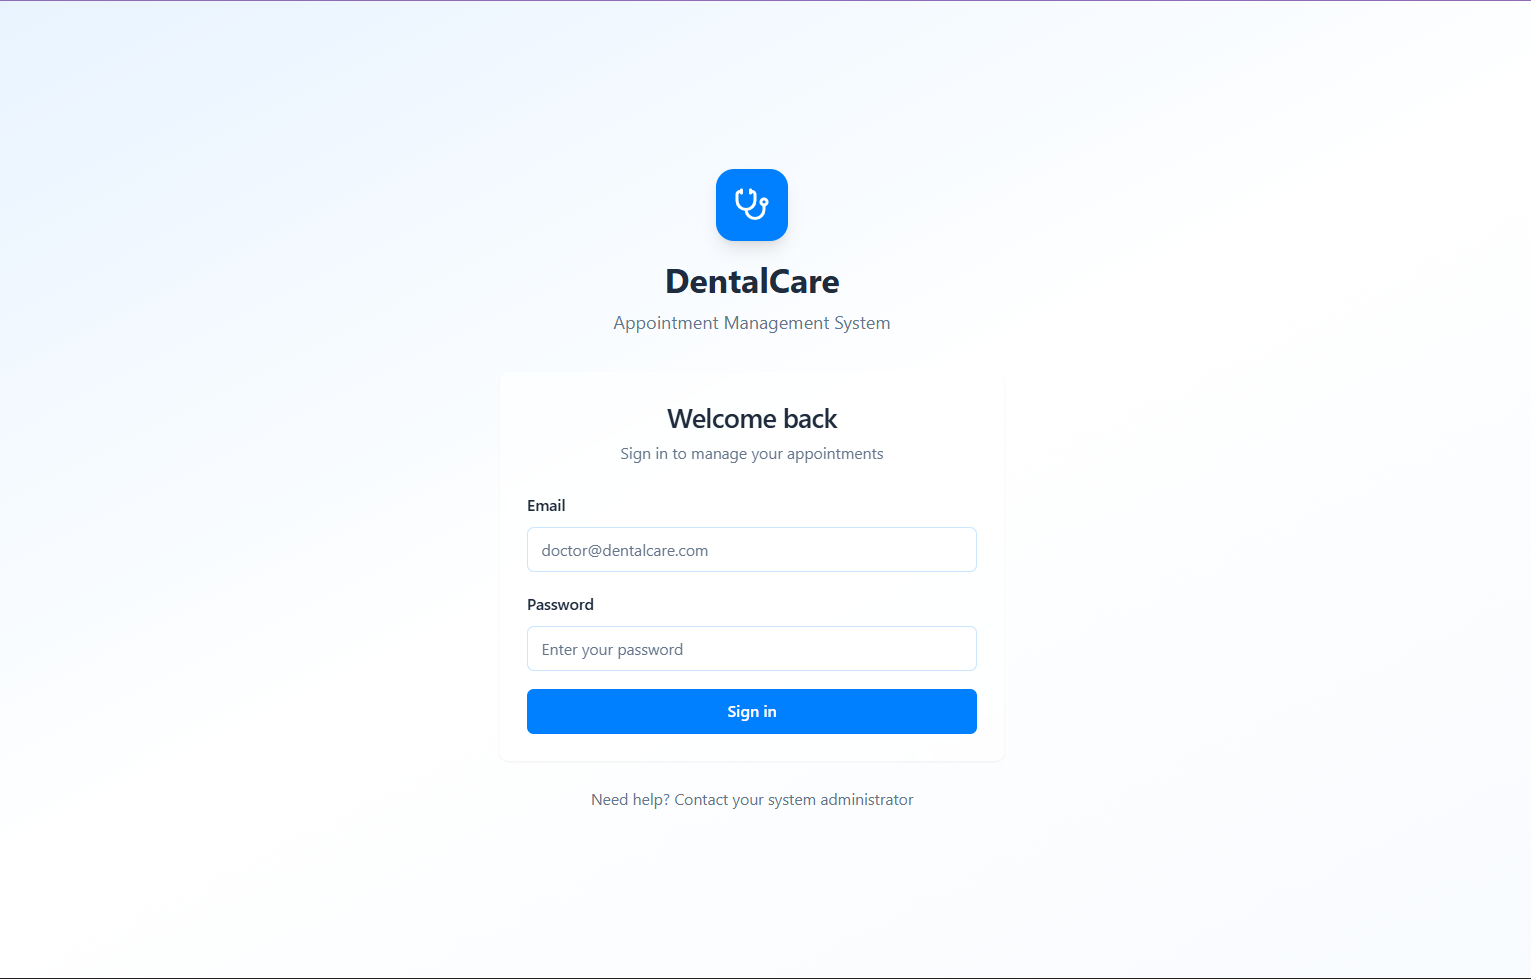
\includegraphics[width=0.8\textwidth]{screenshot_login.png}
 \caption{Capture d'écran~: Page de connexion}
 \label{fig:screenshot_login}
 \end{figure}

La page de connexion (\texttt{Login.tsx}) présente~:
\begin{itemize}
    \item Un arrière-plan avec dégradé bleu-violet et effet glassmorphism
    \item Une carte centrale avec logo \og DentalCare \fg, champ email, champ mot de passe
    \item Bouton \og Sign in \fg{} avec animation de chargement (spinner)
    \item Gestion d'erreurs via notification toast rouge
    \item Redirection automatique vers \texttt{/dashboard} après succès
\end{itemize}

\subsection{Tableau de bord (Dashboard)}

 \begin{figure}[H]
 \centering
 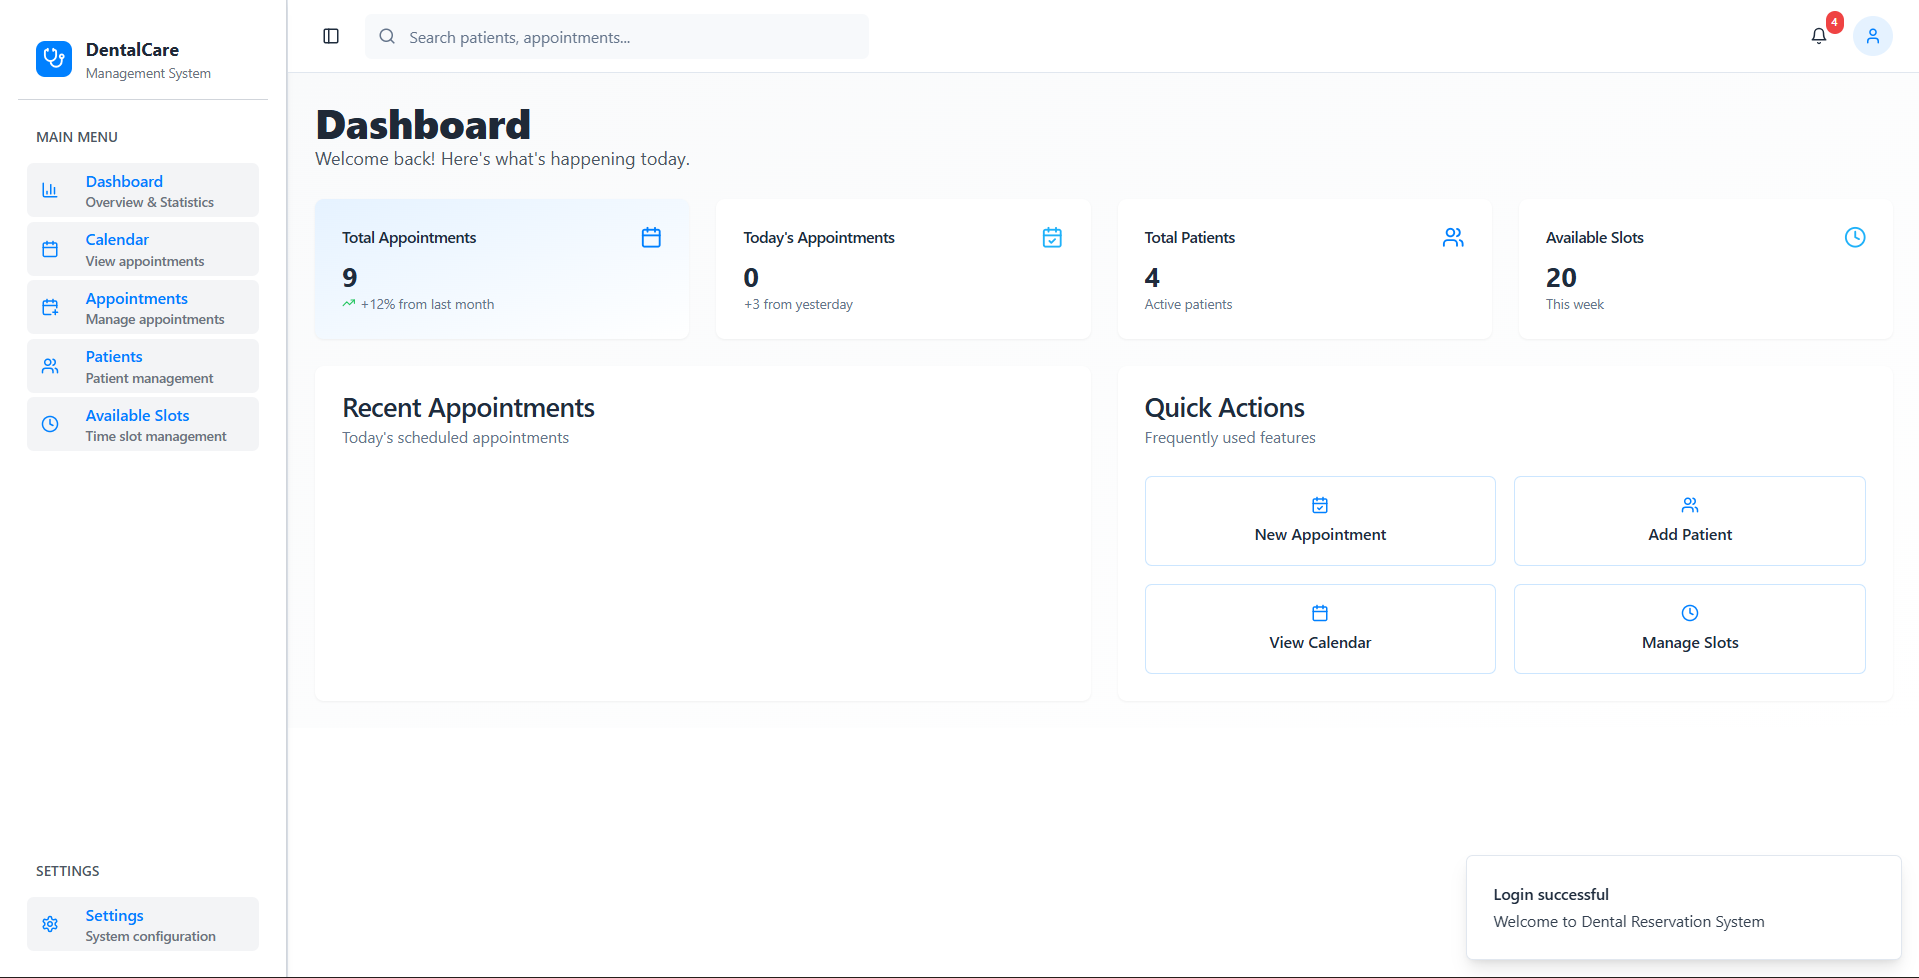
\includegraphics[width=0.85\textwidth]{screenshot_dashboard.png}
 \caption{Capture d'écran~: Tableau de bord}
 \label{fig:screenshot_dashboard}
 \end{figure}

Le Dashboard (\texttt{Dashboard.tsx}) affiche~:

\textbf{4 cartes de statistiques~:}
\begin{table}[H]
\centering
\begin{tabular}{@{} l l l l @{}}
\toprule
\textbf{Carte} & \textbf{Icône} & \textbf{Donnée} & \textbf{Couleur} \\
\midrule
Total Appointments & Calendar & Total RDV en base & Bleu \\
Today's Appointments & Clock & RDV du jour & Vert \\
Total Patients & Users & Patients actifs & Violet \\
Available Slots & CheckCircle & Créneaux libres & Orange \\
\bottomrule
\end{tabular}
\end{table}

\textbf{Section \og Recent Appointments \fg~:} les 6 premiers RDV du jour avec nom, type de soin, heure et badge de statut.

\textbf{Section \og Quick Actions \fg~:} quatre boutons d'accès rapide vers les pages principales.

\subsection{Gestion des patients (Patients)}

 \begin{figure}[H]
 \centering
 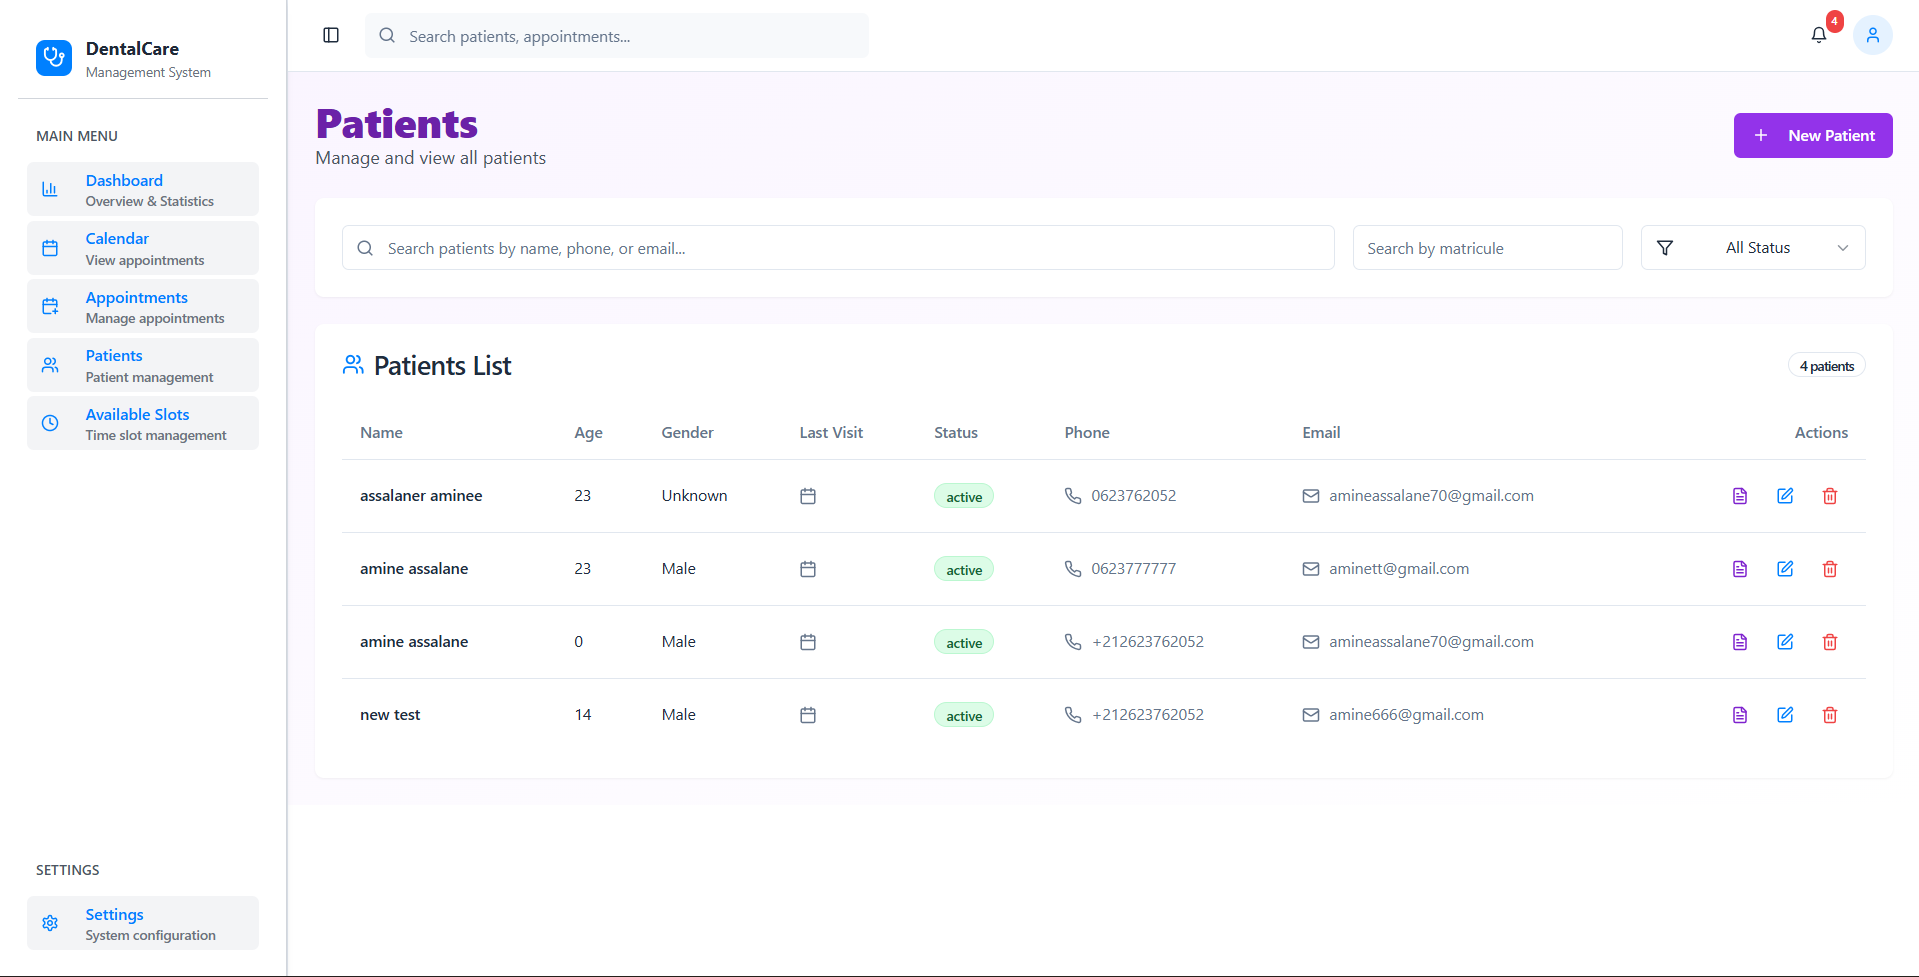
\includegraphics[width=0.85\textwidth]{screenshot_patients.png}
 \caption{Capture d'écran~: Gestion des patients}
 \label{fig:screenshot_patients}
 \end{figure}

La page Patients (\texttt{Patients.tsx}) offre~:
\begin{itemize}
    \item Bouton \og + New Patient \fg{} ouvrant une modale de création
    \item Barre de recherche avec filtrage en temps réel par nom, téléphone, email
    \item Filtres par matricule et par statut (Active, New, Inactive)
    \item Tableau avec colonnes~: Name, Age, Gender, Last Visit, Status, Phone, Email, Actions
    \item Actions par ligne~: Dossier, Éditer, Supprimer
    \item Modale de création/édition avec 16 champs
\end{itemize}

\subsection{Gestion des rendez-vous (Appointments)}

 \begin{figure}[H]
 \centering
 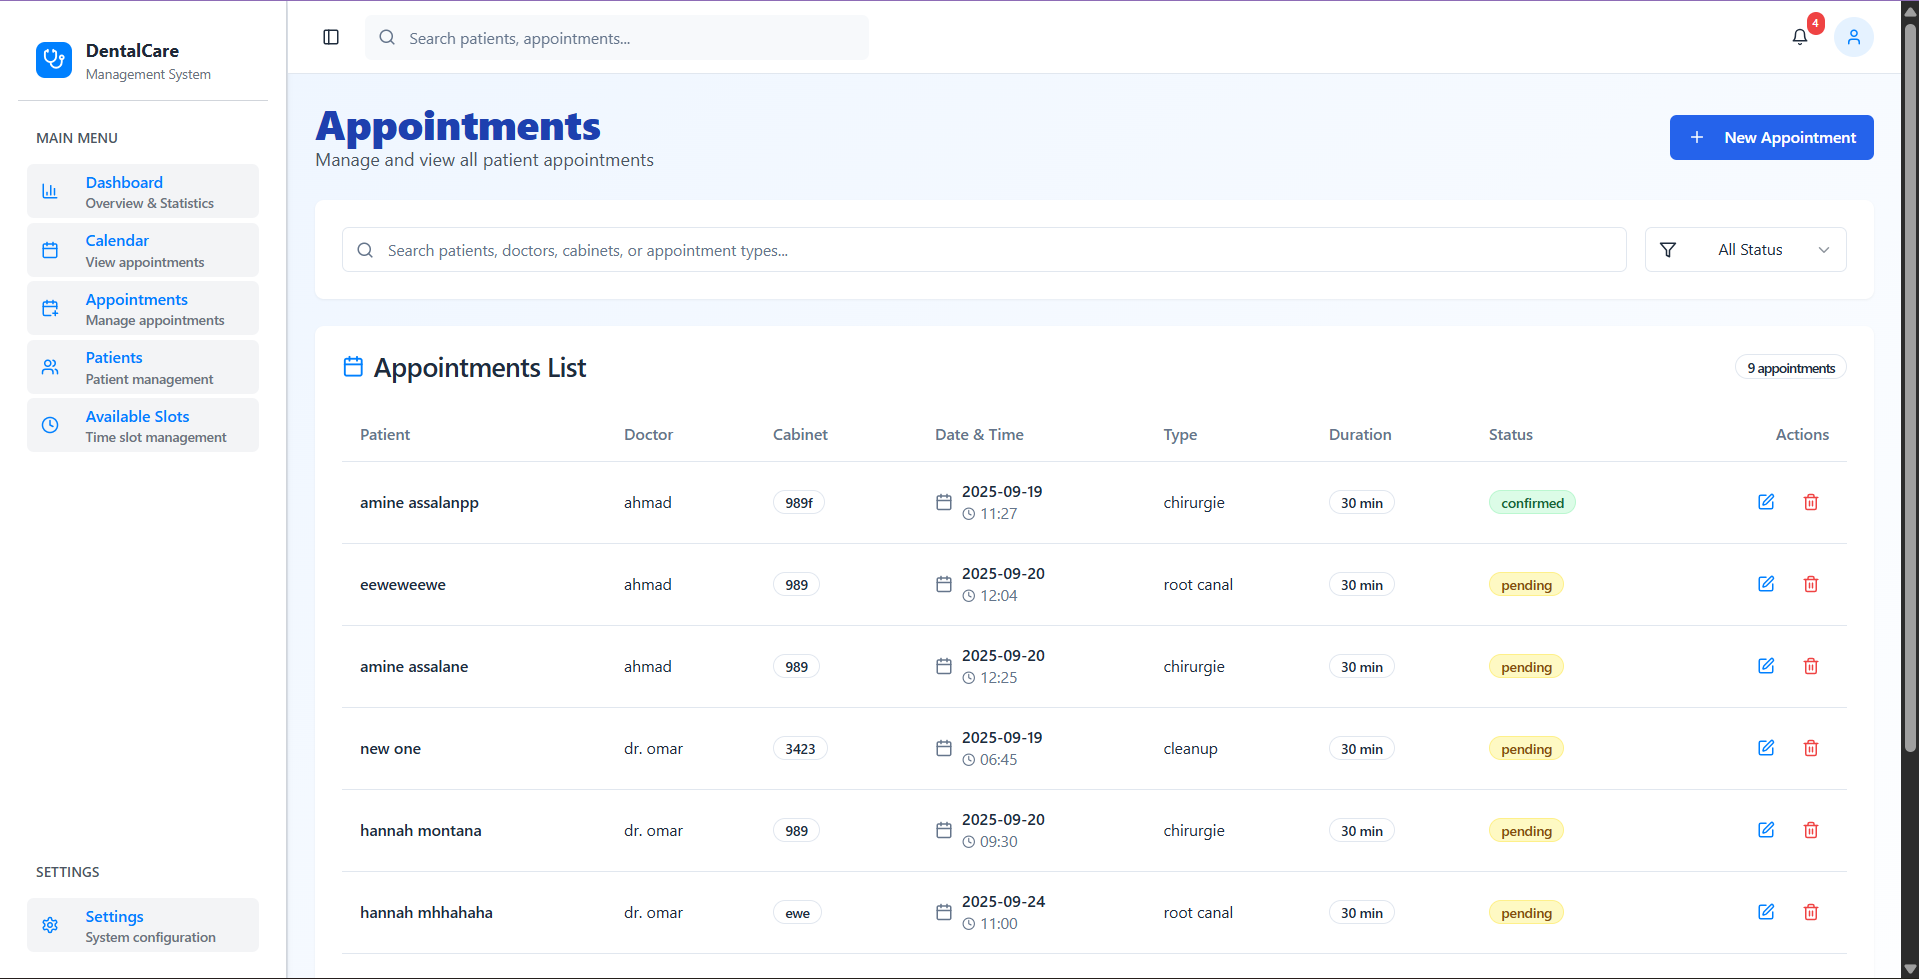
\includegraphics[width=0.85\textwidth]{screenshot_appointments.png}
 \caption{Capture d'écran~: Gestion des rendez-vous}
 \label{fig:screenshot_appointments}
 \end{figure}

La page Appointments (\texttt{Appointments.tsx}) offre~:
\begin{itemize}
    \item Bouton \og + New Appointment \fg{} avec modale contenant~:
    \begin{itemize}
        \item Sélecteur de patient (Combobox recherchable avec nom + matricule)
        \item Champs~: médecin, cabinet, date, heure, durée (15/30/45/60 min), statut, nature du soin, notes
    \end{itemize}
    \item Filtre par statut (Confirmed, Pending, Canceled)
    \item Tableau~: Patient, Doctor, Cabinet, Date \& Time, Type, Duration, Status, Actions
    \item Badges colorés selon le statut (vert/jaune/rouge)
\end{itemize}

\subsection{Calendrier hebdomadaire (Calendar)}

 \begin{figure}[H]
 \centering
 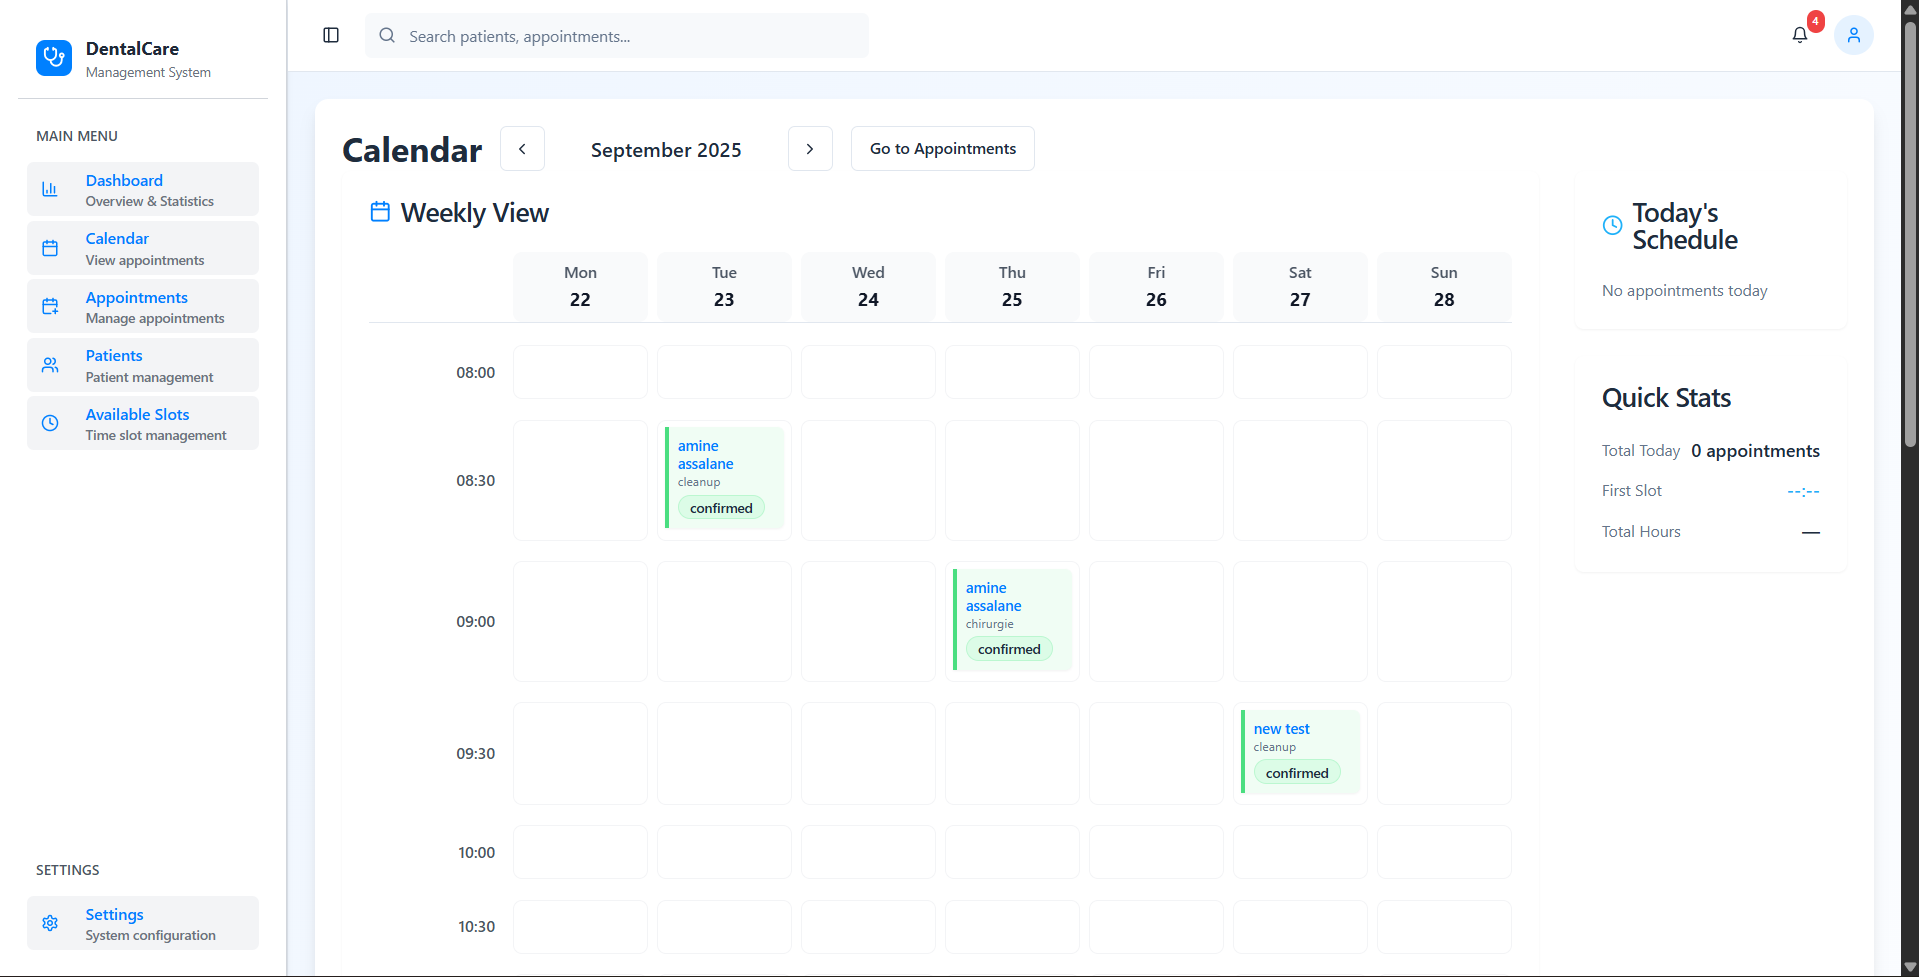
\includegraphics[width=0.85\textwidth]{screenshot_calendar.png}
 \caption{Capture d'écran~: Calendrier hebdomadaire}
 \label{fig:screenshot_calendar}
 \end{figure}

La page Calendar (\texttt{Calendar.tsx}) présente~:
\begin{itemize}
    \item Navigation semaine par semaine avec boutons précédent/suivant
    \item Grille 8 colonnes (heure + 7 jours) $\times$ 20 lignes (08:00 à 17:30, pas de 30 min)
    \item En-têtes des jours avec mise en surbrillance du jour courant
    \item Rendez-vous dans les cellules avec bordure latérale colorée selon le statut
    \item Indicateur rouge de l'heure courante sur la colonne du jour
    \item Panneau latéral \og Today's Schedule \fg{} avec les RDV du jour
    \item Panneau \og Quick Stats \fg{} (total du jour, premier créneau)
\end{itemize}

\subsection{Créneaux disponibles (Available Slots)}

 \begin{figure}[H]
 \centering
 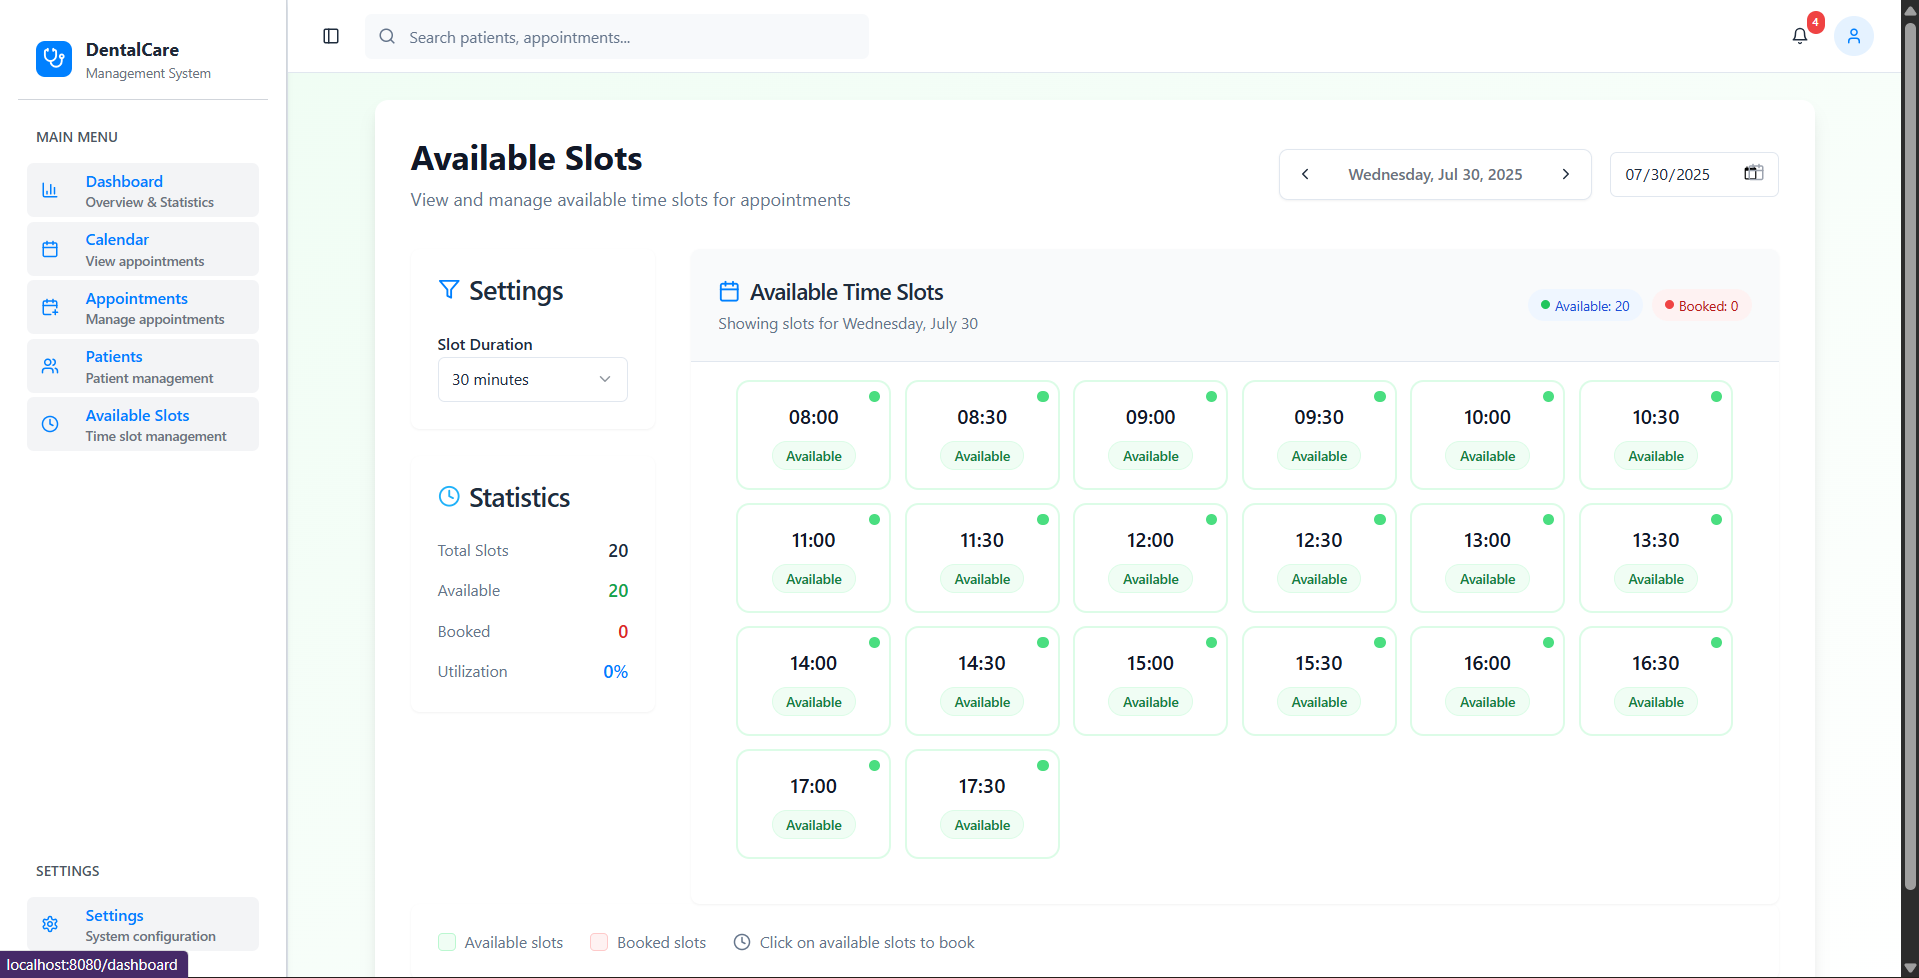
\includegraphics[width=0.85\textwidth]{screenshot_slots.png}
 \caption{Capture d'écran~: Créneaux disponibles}
 \label{fig:screenshot_slots}
 \end{figure}

La page Available Slots (\texttt{AvailableSlots.tsx}) affiche~:
\begin{itemize}
    \item Navigation par jour avec boutons et sélecteur de date
    \item Panneau de configuration~: durée du créneau (15/30/45/60 min), statistiques (total, disponibles, réservés, taux d'utilisation)
    \item Grille responsive de créneaux~: vert = disponible (cliquable), gris = réservé
    \item Modale de réservation rapide au clic sur un créneau disponible
\end{itemize}

\subsection{Dossier patient (Patient Dossier)}

 \begin{figure}[H]
 \centering
 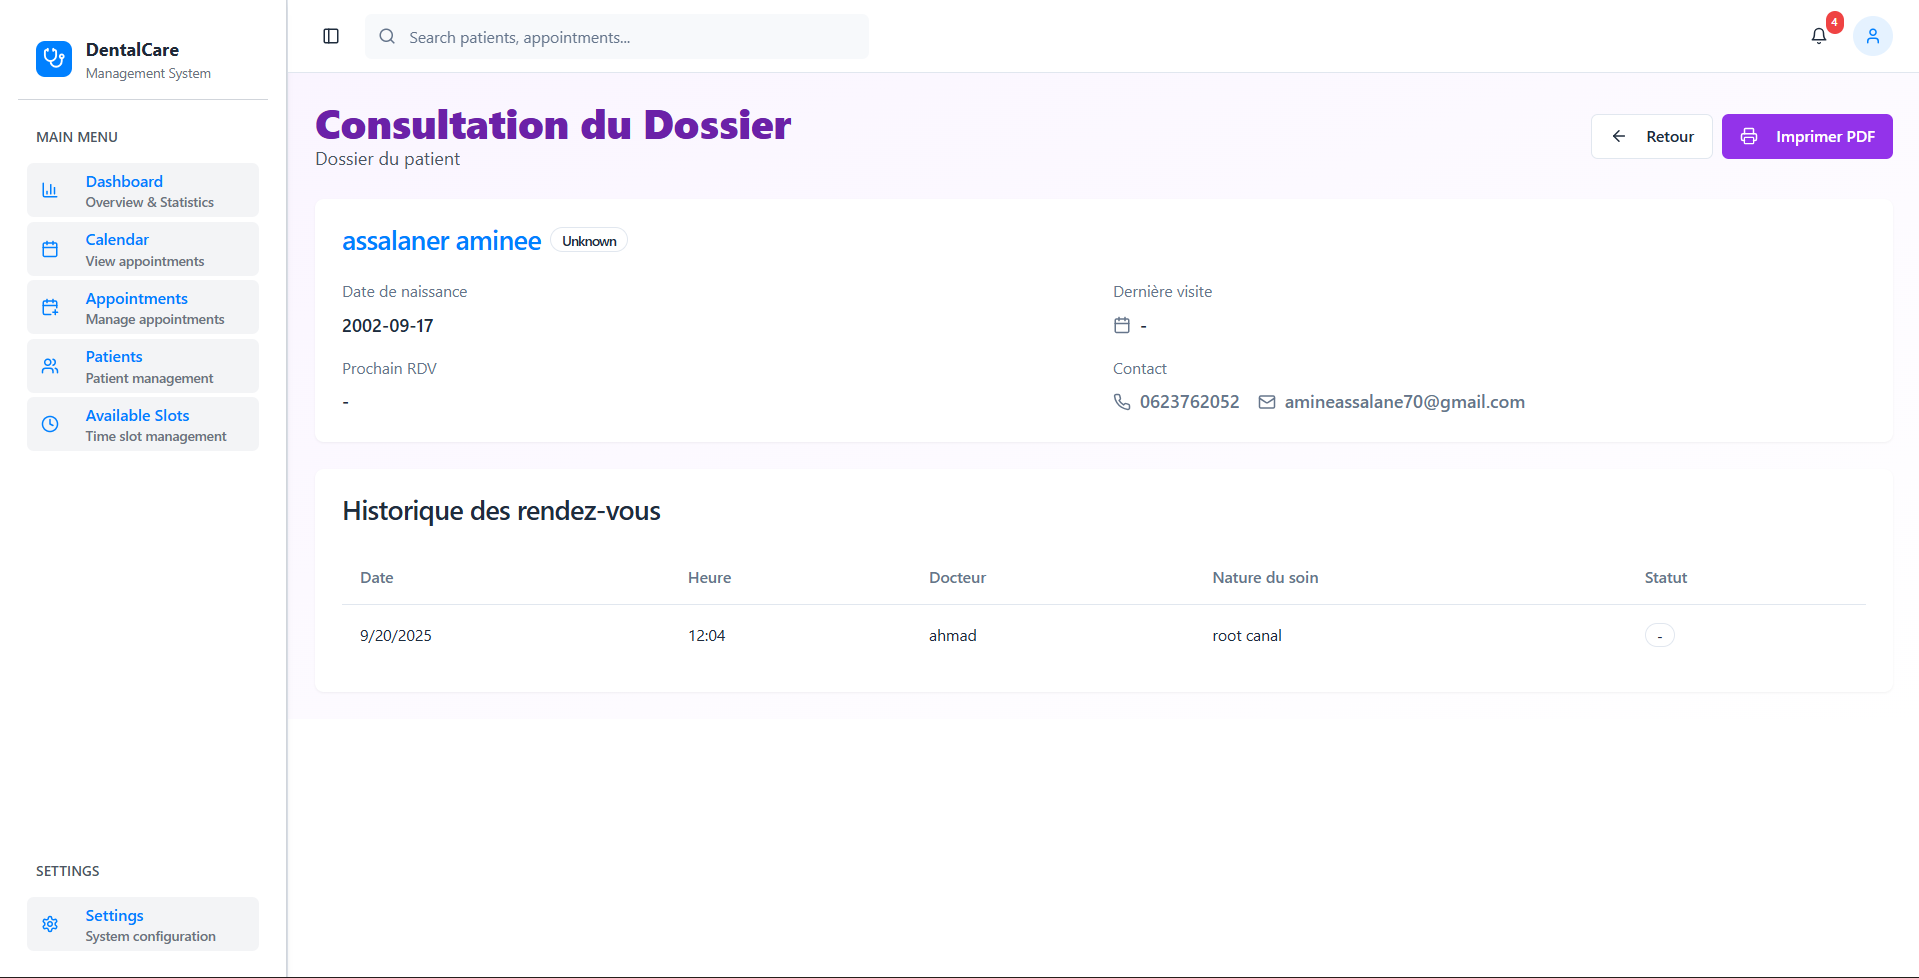
\includegraphics[width=0.85\textwidth]{screenshot_dossier.png}
 \caption{Capture d'écran~: Dossier patient}
 \label{fig:screenshot_dossier}
 \end{figure}

La page PatientDossier (\texttt{PatientDossier.tsx}) affiche~:
\begin{itemize}
    \item En-tête avec nom du patient, badge de genre, bouton retour et bouton \og Imprimer PDF \fg
    \item Carte d'informations~: date de naissance, dernière visite, prochain RDV, téléphone, email
    \item Tableau d'historique des rendez-vous (date, heure, docteur, nature du soin, statut)
    \item Export PDF via \texttt{window.print()} avec feuille de style \texttt{@media print} dédiée
\end{itemize}

\subsection{Profil utilisateur (Profile)}

 \begin{figure}[H]
 \centering
 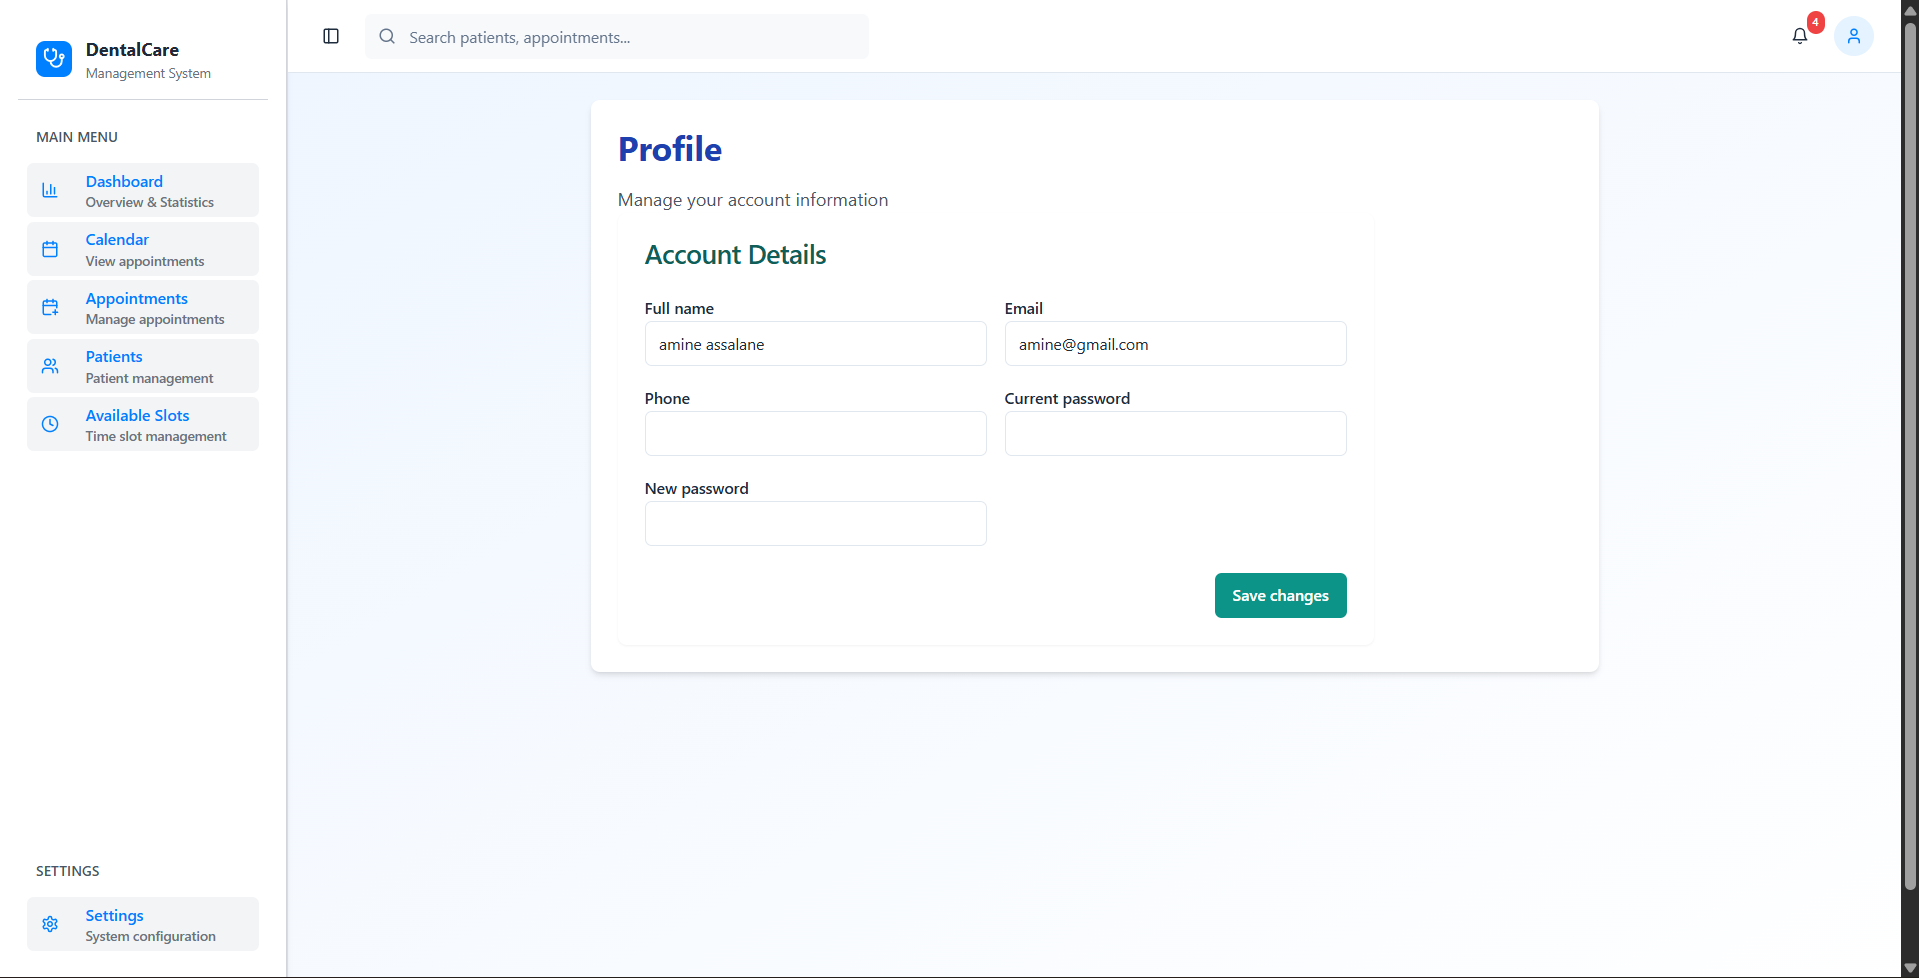
\includegraphics[width=0.7\textwidth]{screenshot_profile.png}
 \caption{Capture d'écran~: Page de profil}
 \label{fig:screenshot_profile}
 \end{figure}

La page Profile (\texttt{Profile.tsx}) permet~:
\begin{itemize}
    \item Section \og Profile Information \fg~: email (lecture seule), nom (modifiable)
    \item Section \og Change Password \fg~: ancien mot de passe + nouveau mot de passe
    \item Données chargées via \texttt{GET /api/Profile/me}, modifications via \texttt{PUT}
\end{itemize}

\subsection{Navigation et mise en page}

\textbf{Barre latérale} (\texttt{AppSidebar.tsx})~:
\begin{itemize}
    \item Logo \og DentalCare Pro \fg{} en en-tête
    \item Menu~: Dashboard, Calendar, Appointments, Patients, Available Slots, Settings
    \item Mode rétractable (icône seule)
    \item Mise en surbrillance de la page active via \texttt{useLocation}
\end{itemize}

\textbf{Barre de navigation supérieure} (\texttt{DashboardLayout.tsx})~:
\begin{itemize}
    \item Bouton de rétraction de la sidebar
    \item Barre de recherche globale
    \item Bouton de notifications avec badge de compteur et panneau déroulant
    \item Menu utilisateur (DropdownMenu)~: nom du praticien, lien Profil, bouton Logout
\end{itemize}

% ============================================================
\section{Conclusion}

La phase de réalisation a permis de livrer une application fonctionnelle couvrant l'ensemble des besoins exprimés. Les fonctionnalités clés --- authentification sécurisée, gestion CRUD des patients et des rendez-vous, détection de conflits, calendrier hebdomadaire, créneaux disponibles et profil utilisateur --- sont pleinement opérationnelles.

L'architecture choisie (API REST + SPA React) offre une séparation claire des responsabilités et une expérience utilisateur fluide grâce au rendu côté client, au cache React Query et aux notifications toast instantanées.

% ============================================================
%  Conclusion Générale et Perspectives
%  Titre : gras centré 24pt Times New Roman
% ============================================================
\clearpage
\thispagestyle{plain}

\vspace*{2cm}

\begin{center}
{\fontsize{24}{29}\selectfont\bfseries Conclusion Générale et Perspectives}
\end{center}
\addcontentsline{toc}{chapter}{Conclusion Générale et Perspectives}

\vspace{1.5cm}

Le projet \textbf{Dental Reservation} a permis de concevoir et réaliser une solution web complète, moderne et fonctionnelle pour la gestion des cabinets dentaires. L'application couvre l'ensemble du cycle de gestion~: de l'authentification sécurisée du praticien, à la gestion des patients et de leurs dossiers médicaux, en passant par la planification intelligente des rendez-vous avec détection automatique des conflits de créneaux.

Le choix d'une architecture client-serveur avec un backend ASP.NET Core 8 et un frontend React TypeScript a permis une séparation claire des responsabilités, facilitant la maintenance et l'évolution du système. L'utilisation d'Entity Framework Core comme ORM a simplifié les interactions avec la base de données SQL Server tout en protégeant contre les injections SQL. TanStack React Query a optimisé la gestion de l'état serveur côté frontend, offrant un cache intelligent et une synchronisation automatique.

La modélisation UML réalisée avec PlantUML (8 diagrammes) a fourni une base solide de conception avant l'implémentation, couvrant les cas d'utilisation, les classes, les séquences d'interaction et les flux d'activité.

La conteneurisation avec Docker et Docker Compose assure un déploiement reproductible et portable, et la documentation API via Swagger facilite l'intégration et les tests.

\section*{Perspectives d'évolution}

Plusieurs axes d'amélioration et d'extension sont envisagés pour les versions futures~:

\begin{enumerate}
    \item \textbf{Application mobile}~: Développement d'une application mobile React Native ou Flutter permettant aux patients de prendre rendez-vous directement depuis leur smartphone et de recevoir des rappels.

    \item \textbf{Notifications push et rappels}~: Intégration d'un service d'envoi de rappels par email (via SendGrid) ou SMS (via Twilio) avant chaque rendez-vous, réduisant le taux de rendez-vous manqués.

    \item \textbf{Gestion des paiements et facturation}~: Ajout d'un module de facturation permettant de générer des factures, suivre les paiements et s'intégrer avec des solutions de paiement en ligne.

    \item \textbf{Tableau de bord analytique avancé}~: Intégration de graphiques interactifs avec des bibliothèques comme Recharts ou Chart.js pour visualiser l'évolution des rendez-vous, le taux de remplissage, et les tendances.

    \item \textbf{Multi-cabinet et multi-rôles}~: Support de plusieurs cabinets avec des rôles différenciés (administrateur, praticien, secrétaire, patient) et des permissions granulaires.

    \item \textbf{Intégration avec des systèmes tiers}~: Connexion avec des logiciels de comptabilité, des systèmes d'information hospitaliers (SIH), ou des annuaires de professionnels de santé.

    \item \textbf{Hachage des mots de passe}~: Remplacement du stockage en clair des mots de passe par un algorithme de hachage sécurisé (bcrypt ou Argon2) pour une sécurité renforcée.

    \item \textbf{Tests automatisés}~: Mise en place d'une suite de tests unitaires (xUnit pour le backend, Vitest pour le frontend) et de tests d'intégration pour garantir la fiabilité du code.

    \item \textbf{Internationalisation (i18n)}~: Support multilingue (français, anglais, arabe) pour les cabinets opérant dans des environnements multilingues.

    \item \textbf{Prise de rendez-vous en ligne par les patients}~: Portail web dédié permettant aux patients de consulter les créneaux disponibles et de réserver eux-mêmes leurs rendez-vous.
\end{enumerate}

\clearpage


% ---- Références ----
% ============================================================
%  Références — Titre gras centré 24pt Times New Roman
%  Format : [n] Auteurs, « Titre », Edition/Journal, année, pages
%  Pour sites web : Titre, Lien, consulté le ...
% ============================================================
\clearpage
\thispagestyle{plain}

\vspace*{2cm}

\begin{center}
{\fontsize{24}{29}\selectfont\bfseries Références}
\end{center}
\addcontentsline{toc}{chapter}{Références}

\vspace{1.5cm}

\begin{enumerate}[label={[\arabic*]}]
    \item Microsoft, \og ASP.NET Core Documentation \fg{},\\
    \url{https://learn.microsoft.com/en-us/aspnet/core/}, consulté le 15 janvier 2026.

    \item Microsoft, \og Entity Framework Core Documentation \fg{},\\
    \url{https://learn.microsoft.com/en-us/ef/core/}, consulté le 15 janvier 2026.

    \item React Team, \og React Documentation \fg{},\\
    \url{https://react.dev/}, consulté le 10 janvier 2026.

    \item Vite Team, \og Vite Documentation \fg{},\\
    \url{https://vitejs.dev/}, consulté le 10 janvier 2026.

    \item TailwindCSS Team, \og Tailwind CSS Documentation \fg{},\\
    \url{https://tailwindcss.com/docs}, consulté le 10 janvier 2026.

    \item shadcn, \og shadcn/ui Documentation \fg{},\\
    \url{https://ui.shadcn.com/}, consulté le 12 janvier 2026.

    \item TanStack, \og React Query Documentation \fg{},\\
    \url{https://tanstack.com/query/latest}, consulté le 12 janvier 2026.

    \item Microsoft, \og SQL Server Documentation \fg{},\\
    \url{https://learn.microsoft.com/en-us/sql/}, consulté le 15 janvier 2026.

    \item Docker Inc., \og Docker Documentation \fg{},\\
    \url{https://docs.docker.com/}, consulté le 18 janvier 2026.

    \item Auth0, \og Introduction to JSON Web Tokens \fg{},\\
    \url{https://jwt.io/introduction}, consulté le 20 janvier 2026.

    \item PlantUML, \og PlantUML Documentation \fg{},\\
    \url{https://plantuml.com/}, consulté le 22 janvier 2026.

    \item Radix UI, \og Radix UI Primitives \fg{},\\
    \url{https://www.radix-ui.com/}, consulté le 12 janvier 2026.

    \item Lucide, \og Lucide Icons \fg{},\\
    \url{https://lucide.dev/}, consulté le 12 janvier 2026.
\end{enumerate}

\clearpage


% ---- Annexes ----
% ============================================================
%  Annexes — Titre gras centré 24pt Times New Roman
% ============================================================
\clearpage
\thispagestyle{plain}

\vspace*{2cm}

\begin{center}
{\fontsize{24}{29}\selectfont\bfseries Annexes}
\end{center}
\addcontentsline{toc}{chapter}{Annexes}

\vspace{1.5cm}

\section*{A.1~~Structure du projet}

L'arborescence complète du projet \textbf{Dental Reservation} est organisée comme suit~:

\begin{lstlisting}[language={}, caption={Arborescence du projet}]
Dental-reservation/
  api/                          # Backend ASP.NET Core 8
    Controllers/                # 7 controleurs REST
    Models/                     # 8 entites + DTOs
    Data/                       # ApplicationDbContext
    Program.cs                  # Point d'entree
    appsettings.json            # Configuration
    Dockerfile                  # Build multi-stage
  frontend/                     # Frontend React 18
    src/
      pages/                    # 8 pages
      components/               # Composants UI
      hooks/                    # 3 hooks personnalises
      lib/                      # ApiService + utils
    vite.config.ts              # Configuration Vite
    tailwind.config.ts          # Configuration Tailwind
    Dockerfile                  # Build multi-stage + Nginx
  docker-compose.yml            # Orchestration
  diagrams/                     # 8 diagrammes PlantUML
\end{lstlisting}

\section*{A.2~~Configuration Docker Compose}

Le fichier \texttt{docker-compose.yml} orchestre les deux services de l'application~:

\begin{lstlisting}[language=yaml, caption={docker-compose.yml}]
version: "3.8"
services:
  api:
    build:
      context: ./api
      dockerfile: Dockerfile
    ports:
      - "5057:8080"
    environment:
      - ASPNETCORE_ENVIRONMENT=Production
  frontend:
    build:
      context: ./frontend
      dockerfile: Dockerfile
    ports:
      - "80:80"
    depends_on:
      - api
\end{lstlisting}

\section*{A.3~~Fichiers PlantUML}

Les 8 diagrammes UML du projet sont disponibles dans le dossier \texttt{diagrams/}~:

\begin{enumerate}
    \item \texttt{use\_case\_diagram.puml} --- Diagramme de cas d'utilisation
    \item \texttt{class\_diagram.puml} --- Diagramme de classes
    \item \texttt{sequence\_authentification.puml} --- Séquence d'authentification
    \item \texttt{sequence\_rendez\_vous.puml} --- Séquence de gestion des rendez-vous
    \item \texttt{sequence\_patients.puml} --- Séquence de gestion des patients
    \item \texttt{activity\_authentification.puml} --- Activité d'authentification
    \item \texttt{activity\_rendez\_vous.puml} --- Activité de création d'un rendez-vous
    \item \texttt{activity\_patients.puml} --- Activité de gestion des patients (CRUD)
\end{enumerate}

\clearpage


\end{document}
